%페이지 세팅
% 한국어 Setting의 경우 10 pt 이용해주자. 또한 줄간격인 line spread 도 1.15로 설정 
\documentclass[9.2pt,a4paper]{article}
\setlength{\parindent}{0em}                  %DISTANCIA SANGRÍA
\setlength{\parskip}{0.5em}                  %DISTANCIA ENTRE PÁRRAFOS
\linespread{1.2}
\textwidth 6.5in
\textheight 9.in
\oddsidemargin 0in
\headheight 0in
\usepackage{amsmath}
\usepackage{tcolorbox}
\usepackage{amssymb}
\usepackage{amsthm}
\usepackage{lastpage}
\usepackage{fancyhdr}
\usepackage{accents}
\usepackage{setup}
\usepackage{import}
\usepackage{fancyhdr}
\usepackage{layouts}
\addtolength{\voffset}{0mm}
\addtolength{\textheight}{0mm}

\usepackage{xcolor}
\usepackage{mdframed}
\usepackage[shortlabels]{enumitem}
\usepackage{indentfirst}
\usepackage{hyperref}

\setlength{\columnsep}{5mm}

\usepackage{enumitem}
\newlist{enumerateoptional}{enumerate}{1}
\setlist[enumerateoptional]{
    before=\let\item\optionalItem,
    label=\arabic*,
    nosep,
    labelindent=20mm,
    leftmargin=*
}
\makeatletter
%%%%%%%%%%%%%%%%%%%%%%%%%%%%%%%%%%%%%%%%%%%%%%%%%%%%%%%%%%%%%%%%%%%%%%%%%%
% Sectioning Sytle Change
\renewcommand{\thesubsection}{Experiment \thesection-\arabic{subsection}}
\renewcommand{\thesubsubsection}{\thesection. \arabic{subsection}. \arabic{subsubsection}}
% \renewcommand{\thesubsection}{\thesection.\alph{subsection}}
% Customize Section Style
% we use \prefix@<level> only if it is defined
\renewcommand{\@seccntformat}[1]{%
  \ifcsname prefix@#1\endcsname
    \csname prefix@#1\endcsname
  \else
    \csname the#1\endcsname\quad
  \fi}
% define \prefix@section
% 11 / 14 실험 제목 생략을 위해서 잠시 수정해줌 
\newcommand\prefix@section{Experiment  \thesection}
% \newcommand\prefix@subsection{Experiment \thesection-\thesubsection}
% \newcommand\prefix@subsubsection{\quad \thesubsubsection\ \ }
\makeatother
%%%%%%%%%%%%%%%%%%%%%%%%%%%%%%%%%%%%%%%%%%%%%%%%%%%%%%%%%%%%%%%%%%%%%%%%%%
\let\realItem\item
% Setting Table Color
% \usepackage[table,xcdraw]{xcolor}
\newcommand\optionalItem[1][]{%
  \refstepcounter{enumerateoptionali}% increment the counter
  \realItem[\bfseries#1~\theenumerateoptionali)]%
}
% WEEK 06 파이썬 코드 의 listing 을 위해서 수정해주는 이름 부분 
% \usepackage{listings}
% \renewcommand{\lstlistingname}{mininet python API custom code}
% \renewcommand{\figcaption}{\footnotesize \textbf{mininet API} python custom code}
\renewcommand{\listingscaption}{\footnotesize \textbf{OMNet++ Source Code}}

%%%%%%%%%%%%%%%%%%%%%%%%%%%%%%%%%%%%%%%%%%%%%%%%%%%%%%%%%%%%%%%%%%%%%%%%%%
    % 매주 리포트를 작성할때 이 부분을 수정하면 보고서 전체가 수정된다. 
%%%%%%%%%%%%%%%%%%%%%%%%%%%%%%%%%%%%%%%%%%%%%%%%%%%%%%%%%%%%%%%%%%%%%%%%%%
% 작성하는 주차
\newcommand{\numnum}{13}
% 실험 부제목
% \newcommand{\subtitle}{wireshark(1) : Getting started HTTP DNS}
% \newcommand{\subtitle}{wireshark(2) : TCP UDP IP protocols}
% \newcommand{\subtitle}{USPR(1) : Introduction, Labview, Spectogram}
% \newcommand{\subtitle}{USPR(2) : Active Sensing}
% \newcommand{\subtitle}{USPR(3) : CNN Classifier}
% \newcommand{\subtitle}{mininet (2) : sdn-based Routing}
% \newcommand{\subtitle}{OMNet++ Simulator Basic}
% \newcommand{\subtitle}{Medium Access Control}
\newcommand{\subtitle}{V2X Communication: VANET Tutorial}
%-------------------------------------------------------------------------
%--> 떠다니는 객체 사용하는 부분 
\usepackage{wrapfig}
% --> Problem numbering 부분의 수정 필요 
% \newenvironment{problem}[2][Problem]  
%     { \begin{mdframed}[backgroundcolor=gray!20] \textbf{#1 #2} \\}
%     {  \end{mdframed}}
% Enumerate Listing modified 
% \renewcommand{\labelenumi}{Problem  \theenumi}
\newcommand{\soln}[1][Answer]{\noindent\textbf{#1}\quad}
% \newenvironment{problem}[2][Problem]  
%     { \begin{mdframed}[backgroundcolor=gray!20] \textbf{#1 #2} \\}
%     {  \end{mdframed}}
%-------------------------------------------------------------------------
\begin{document}
\pagestyle{fancy}
\fancyhf{}
    \rhead{\small 2조 2016142096 조윤신, 2017142043 김재민}
    \lhead{\textsc{Result Report Week\ \numnum\ \subtitle}}
\cfoot{\thepage}
\renewcommand\headrulewidth{0.3mm}
%\renewcommand\footrulewidth{0.3mm}
\thispagestyle{plain}
\begin{flushleft}
\textsc{School of Electrical and Electronic of Enginnering} \\
\textsc{eee 4474-01 : Experiments on Communication Networks }\\[0.1cm]
\small{\textsc{\textbf{2조} 2016142096 \textbf{조윤신}, 2017142043 \textbf{김재민}}}\\
\end{flushleft}

\begin{flushright}\vspace{-25mm}
    
\includegraphics[height=3cm]{image/1.jpg}
    \vspace{5mm}
\end{flushright}
    \begin{center}\vspace{-1.5cm}
        \textbf{\huge  Result Report Week \numnum}\\ 
        \vspace{1.8mm}
        {\large \subtitle}\\           
    \end{center}
\vspace{-5mm}
\rule{\linewidth}{0.4mm}
\vspace{-5mm}
%-------------------------------------------------------------------------
% main documents
% 모든 프로그래밍 편집기 (IDE)에서 원도우 기준으로 '컨트롤 + /'를 누르면 
% 커서가 활성화된 line의 주석처리를 해제 지정할 수 있다. 
%%%%%%%%%%%%%%%%%%%%%%%%%%%%%%%%%%%%%%%%%%%%%%%%%%%%%%%%%%%%%%%%%%%%%%%%%%
                        % For Week 01 ~ 09.14
%%%%%%%%%%%%%%%%%%%%%%%%%%%%%%%%%%%%%%%%%%%%%%%%%%%%%%%%%%%%%%%%%%%%%%%%%%
% \import{./TEX/week01}{01_exp1}
% \import{./TEX/week01}{02_exp2}
% \import{./TEX/week01}{03_exp3}
%-------------------------------------------------------------------------
%%%%%%%%%%%%%%%%%%%%%%%%%%%%%%%%%%%%%%%%%%%%%%%%%%%%%%%%%%%%%%%%%%%%%%%%%%
                        % For Week 02 ~ 09.21
%%%%%%%%%%%%%%%%%%%%%%%%%%%%%%%%%%%%%%%%%%%%%%%%%%%%%%%%%%%%%%%%%%%%%%%%%%
% \import{./TEX/week02}{01_01_tcp}
% \import{./TEX/week02}{01_02_tcp_basic}
% \import{./TEX/week02}{01_03_tcp_congestion}
% \import{./TEX/week02}{02_udp}
% \import{./TEX/week02}{03_01_ip}
% \import{./TEX/week02}{03_02_basic_ipv4}
% \import{./TEX/week02}{03_03_fragmentation}
%-------------------------------------------------------------------------
%%%%%%%%%%%%%%%%%%%%%%%%%%%%%%%%%%%%%%%%%%%%%%%%%%%%%%%%%%%%%%%%%%%%%%%%%%
                        % For Week 03 ~ 09.28
%%%%%%%%%%%%%%%%%%%%%%%%%%%%%%%%%%%%%%%%%%%%%%%%%%%%%%%%%%%%%%%%%%%%%%%%%%
% \import{./TEX/week03}{01-visualization}
% \import{./TEX/week03}{02-tx}
% \import{./TEX/week03}{03-other-txs}
%-------------------------------------------------------------------------
%%%%%%%%%%%%%%%%%%%%%%%%%%%%%%%%%%%%%%%%%%%%%%%%%%%%%%%%%%%%%%%%%%%%%%%%%%
                        % For Week 04 ~ 10.05
%%%%%%%%%%%%%%%%%%%%%%%%%%%%%%%%%%%%%%%%%%%%%%%%%%%%%%%%%%%%%%%%%%%%%%%%%%
% \import{./TEX/week04}{00_notice}
% \import{./TEX/week04}{01-spectrogram}
% \newpage
% \import{./TEX/week04}{02_}
% \newpage
% \import{./TEX/week04}{03_}
%-------------------------------------------------------------------------
%%%%%%%%%%%%%%%%%%%%%%%%%%%%%%%%%%%%%%%%%%%%%%%%%%%%%%%%%%%%%%%%%%%%%%%%%%
                        % For Week 05 ~ 10.12
%%%%%%%%%%%%%%%%%%%%%%%%%%%%%%%%%%%%%%%%%%%%%%%%%%%%%%%%%%%%%%%%%%%%%%%%%%
% \import{./TEX/week05}{00_notice}
% \import{./TEX/week05}{01}
% \import{./TEX/week05}{02}
% \import{./TEX/week05}{03}
% \import{./TEX/week05}{04_01}
% \import{./TEX/week05}{04_02}
%-------------------------------------------------------------------------
%%%%%%%%%%%%%%%%%%%%%%%%%%%%%%%%%%%%%%%%%%%%%%%%%%%%%%%%%%%%%%%%%%%%%%%%%%
                        % For Week 06 ~ 10.26 (중간고사 일정 변경)
%%%%%%%%%%%%%%%%%%%%%%%%%%%%%%%%%%%%%%%%%%%%%%%%%%%%%%%%%%%%%%%%%%%%%%%%%%
% \import{./TEX/week06}{00}
% \import{./TEX/week06}{01}
% \import{./TEX/week06}{02}
% \import{./TEX/week06}{03}
%-------------------------------------------------------------------------
%%%%%%%%%%%%%%%%%%%%%%%%%%%%%%%%%%%%%%%%%%%%%%%%%%%%%%%%%%%%%%%%%%%%%%%%%%
                        % For Week 08 ~ 11.02
%%%%%%%%%%%%%%%%%%%%%%%%%%%%%%%%%%%%%%%%%%%%%%%%%%%%%%%%%%%%%%%%%%%%%%%%%%
% \import{./TEX/week08}{01}
% \import{./TEX/week08}{02}
% \import{./TEX/week08}{03}
% \import{./TEX/week08}{04}
% \import{./TEX/week08}{05}
%-------------------------------------------------------------------------
%%%%%%%%%%%%%%%%%%%%%%%%%%%%%%%%%%%%%%%%%%%%%%%%%%%%%%%%%%%%%%%%%%%%%%%%%%
                        % For Week 09 ~ 11.09
%%%%%%%%%%%%%%%%%%%%%%%%%%%%%%%%%%%%%%%%%%%%%%%%%%%%%%%%%%%%%%%%%%%%%%%%%%
% \import{./TEX/week09}{01}
% \import{./TEX/week09}{02}
% \import{./TEX/week09}{03}
%%%%%%%%%%%%%%%%%%%%%%%%%%%%%%%%%%%%%%%%%%%%%%%%%%%%%%%%%%%%%%%%%%%%%%%%%%
                        % For Week 10 ~ 11.16
%%%%%%%%%%%%%%%%%%%%%%%%%%%%%%%%%%%%%%%%%%%%%%%%%%%%%%%%%%%%%%%%%%%%%%%%%%
% \import{./TEX/week10}{01}
% \import{./TEX/week10}{02}
% \import{./TEX/week10}{03}
%-------------------------------------------------------------------------
%%%%%%%%%%%%%%%%%%%%%%%%%%%%%%%%%%%%%%%%%%%%%%%%%%%%%%%%%%%%%%%%%%%%%%%%%%
                        % For Week 11 ~ 11.23 -> 조윤신 
% notion Link : https://www.notion.so/Week-11-7773a1116c864b7baaafebd13b574259
%%%%%%%%%%%%%%%%%%%%%%%%%%%%%%%%%%%%%%%%%%%%%%%%%%%%%%%%%%%%%%%%%%%%%%%%%%
% \import{./TEX/week11}{01}
% \import{./TEX/week11}{02}
% \import{./TEX/week11}{03}
%-------------------------------------------------------------------------
%%%%%%%%%%%%%%%%%%%%%%%%%%%%%%%%%%%%%%%%%%%%%%%%%%%%%%%%%%%%%%%%%%%%%%%%%%
                        % For Week 12 ~ 11.30 -> 김재민 
                
%%%%%%%%%%%%%%%%%%%%%%%%%%%%%%%%%%%%%%%%%%%%%%%%%%%%%%%%%%%%%%%%%%%%%%%%%%
% \vspace{-6mm}
\section{}
Experiment 1 에서는 MAC (Medium Access Control Layer) 의 contention - based protocol 인 ALOHA의 동작에 대해서 simulation을 진행한다. 
pre report 에서 pure aloha 와 slotted aloha 의 각각 포아송 분포를 가정하는 전송량 G -load 에 따른  이론적인 Throughput의 graph가 각각 $G\times e^{-G},\ G\times e^{-2G}$   를 확인한것과 같이, omnetpp simulatino 을 통해서 pure aloha 와 slotted aloha 각각의   G-load 가 일반의 경우와  optimal인 경우 4가지에 대한  simulation을 진행한다.
\vspace{-2mm}
\subsection{}
    \vspace{-2mm}
    \subsubsection{ini simulation file setting}
    \vspace{-2mm}
    4개의 simulation setting code는 다음과 같다. 각각의 G-load 를 iaTime variable을 통해서 설정한것을 확인할 수 있다.
            \vspace{-2mm}
            \begin{listing}[h!]
            \inputminted[framerule = 1pt,framesep = 2mm , frame = lines, fontsize=\scriptsize ]{c}{./code/week12/Experiment_01/ini.cpp}
            \vspace{-3mm}
            \caption{\footnotesize aloha ini file}
            \end{listing}
            \vspace{-6mm}
    \subsubsection{Simulation Results : Sequence Chart}
    \vspace{-3mm}
    Aloha의 실험결과로 각 simulatino Time 기준으로 10초를 진행하여 생성한 event log를 바탕으로 sequence log와 scalar file 로부터 channel util($\sim$ Throughput) 값을 얻을 수 있었다.
    
    결과 차트는 아래와 같다. 1번쨰 2번째는 Pure Aloha의 G-load 1/6 과 optimal 인 1/2 의 결과로 총 3 sec 가 표기되도록 sequence log 차트의screenshot을 캡처했다. G-load가 3배가 더 만큼 동일시간 동안 3배 더많은 전송이 진행된 것과 pure aloha의 특성상 전송시간이 fix 되지않아 많은 collision이 발생한것을 확인할 수 있다.
    
    3번째, 4번째 Slotted Alohs의 G-load가 1/4 와 optimal 인 1 의 결과로 총 2 sec가 표기되도록 sequence log 차트의screenshot을 캡처했다. 마찬가지로 G-load가 4배 정도 차이가 있지만 slot동안 전송이 요청되는 frame 에 대해서 slot과 slot 사이에서만 전송되는 slotted aloha 의 workflow를 확인할 수 있었고, 각각 pure aloha 보다 collision이 현격히 감소한 것을 확인할 수 있었다. 구체적인 수치는 scalar file에서 확인한 채널효율로 비교해보고자 한다. 
    \clearpage
        \begin{figure}[h!]
        \centering
        \subfloat[Aloha, frequent transmission (high collision rate)]{
            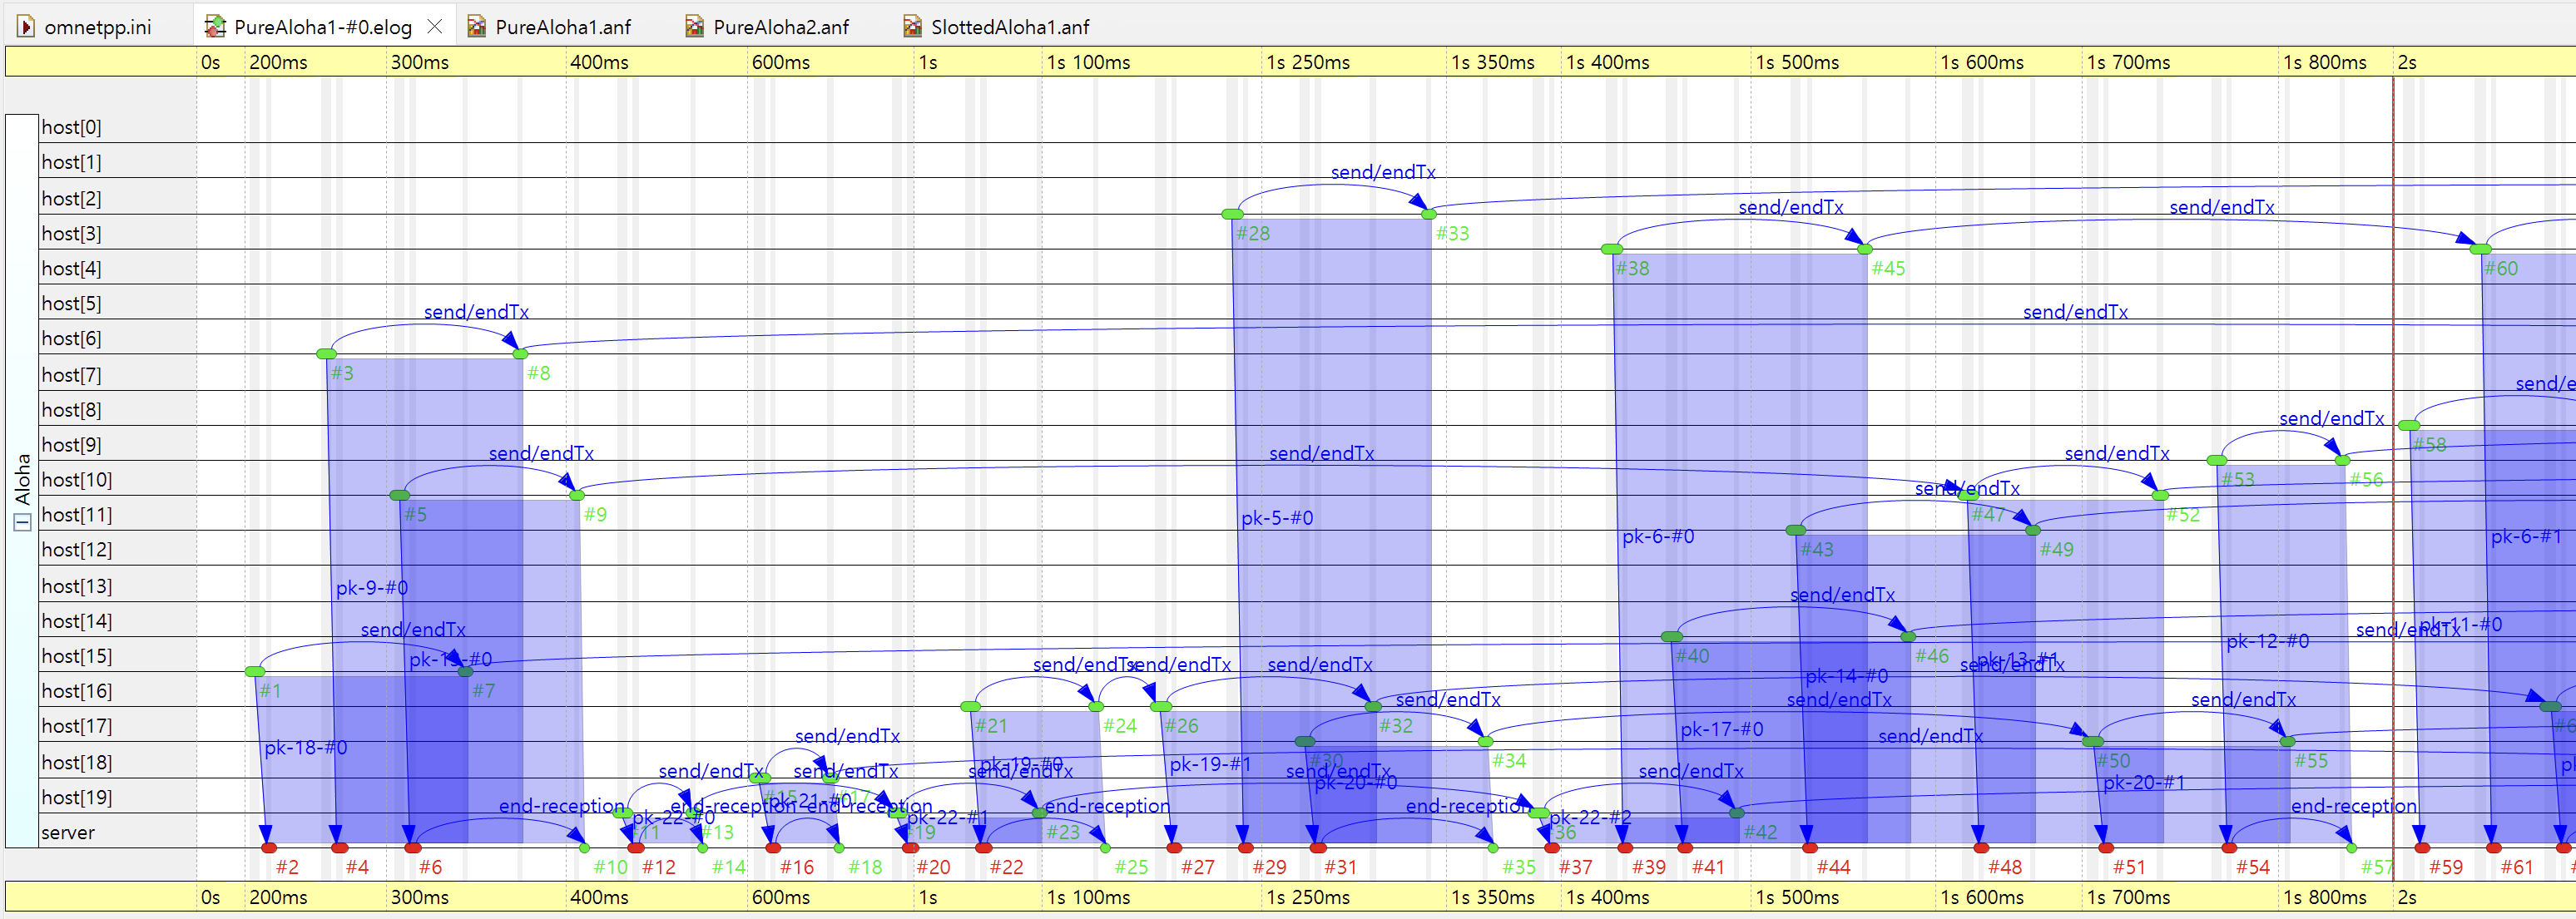
\includegraphics[width=0.93\textwidth]{image/week12/1-1-1.png}
        }\hspace{3mm}
        \subfloat[Aloha, optimal load]{
            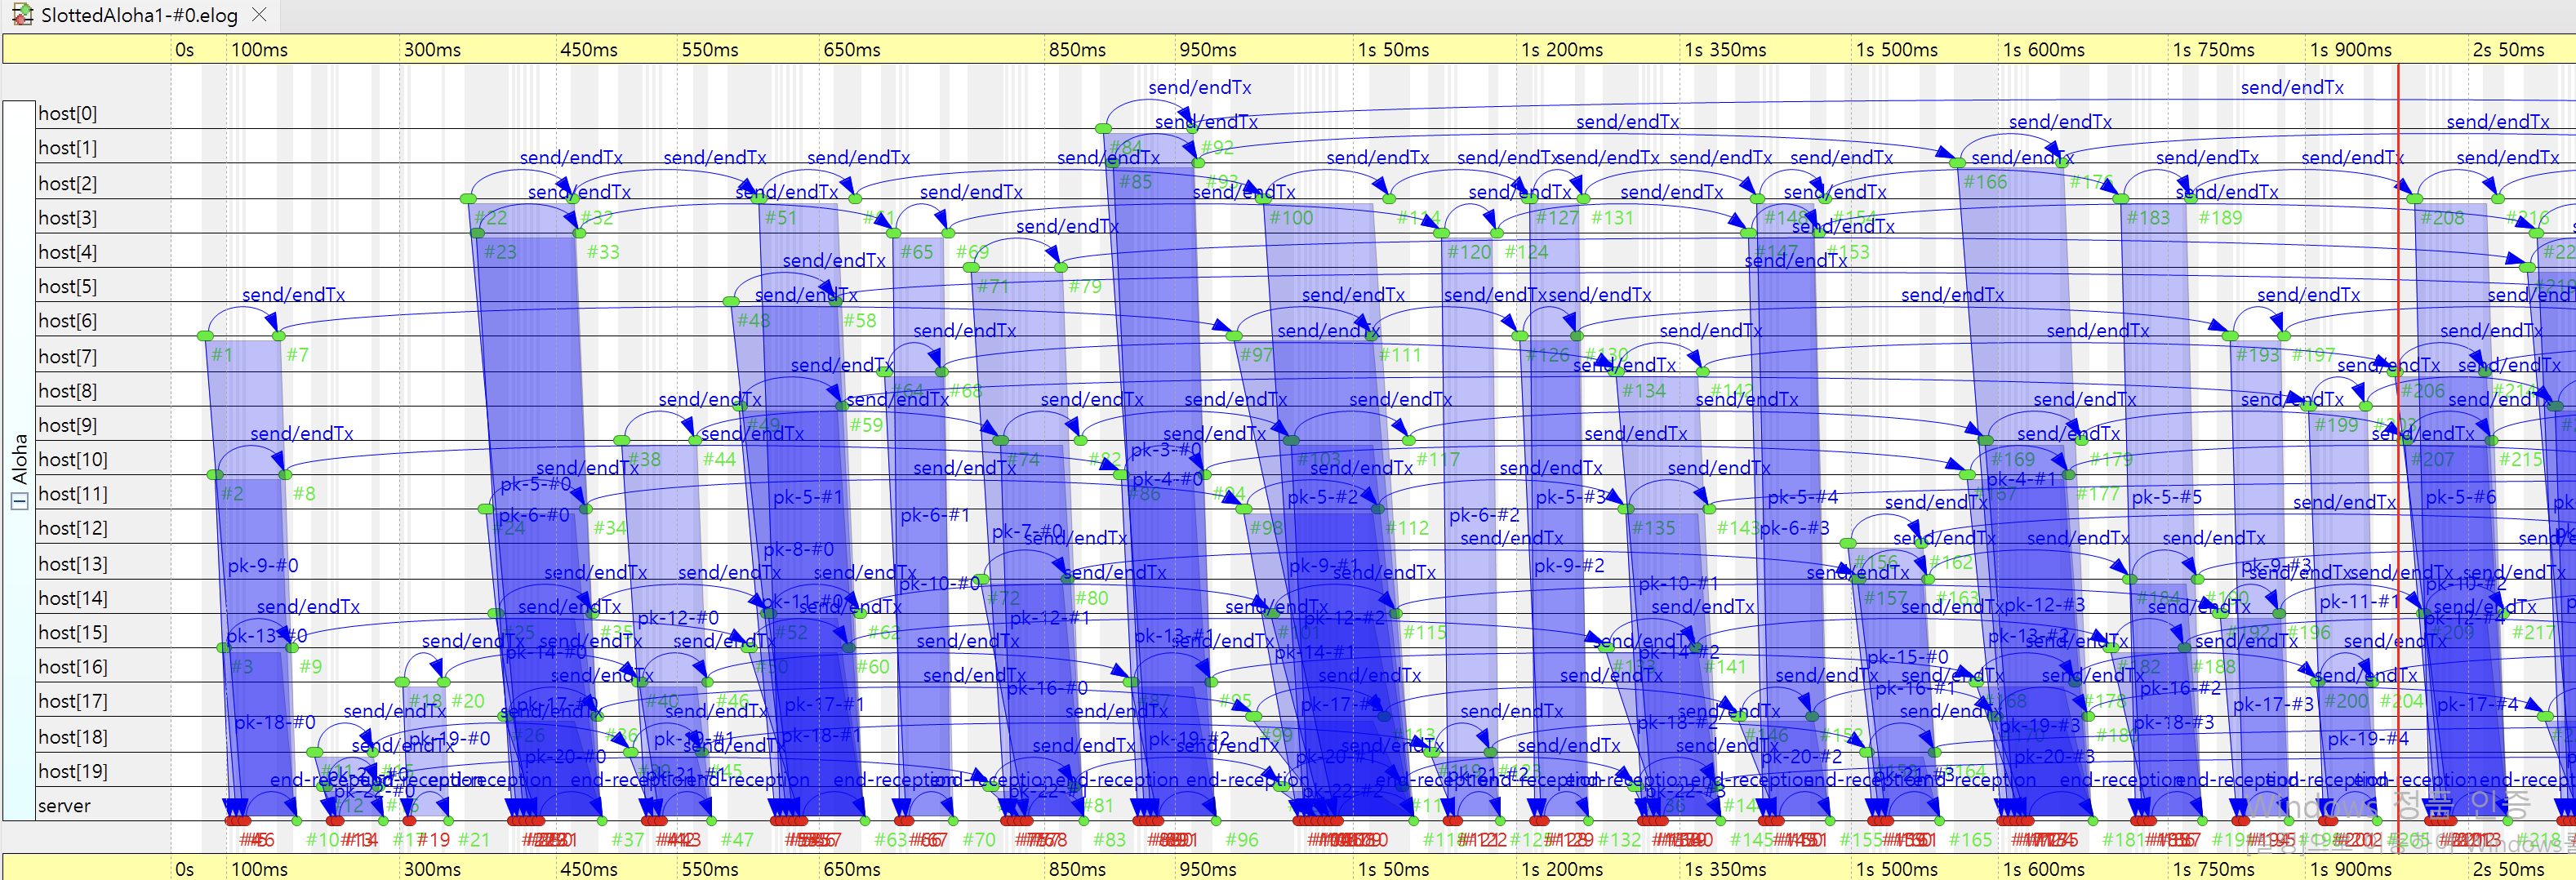
\includegraphics[width=0.93\textwidth]{image/week12/1-1-2.png}
        }\hspace{3mm}
        \subfloat[Slotted Aloha, frequent transmission (high collision rate)]{
            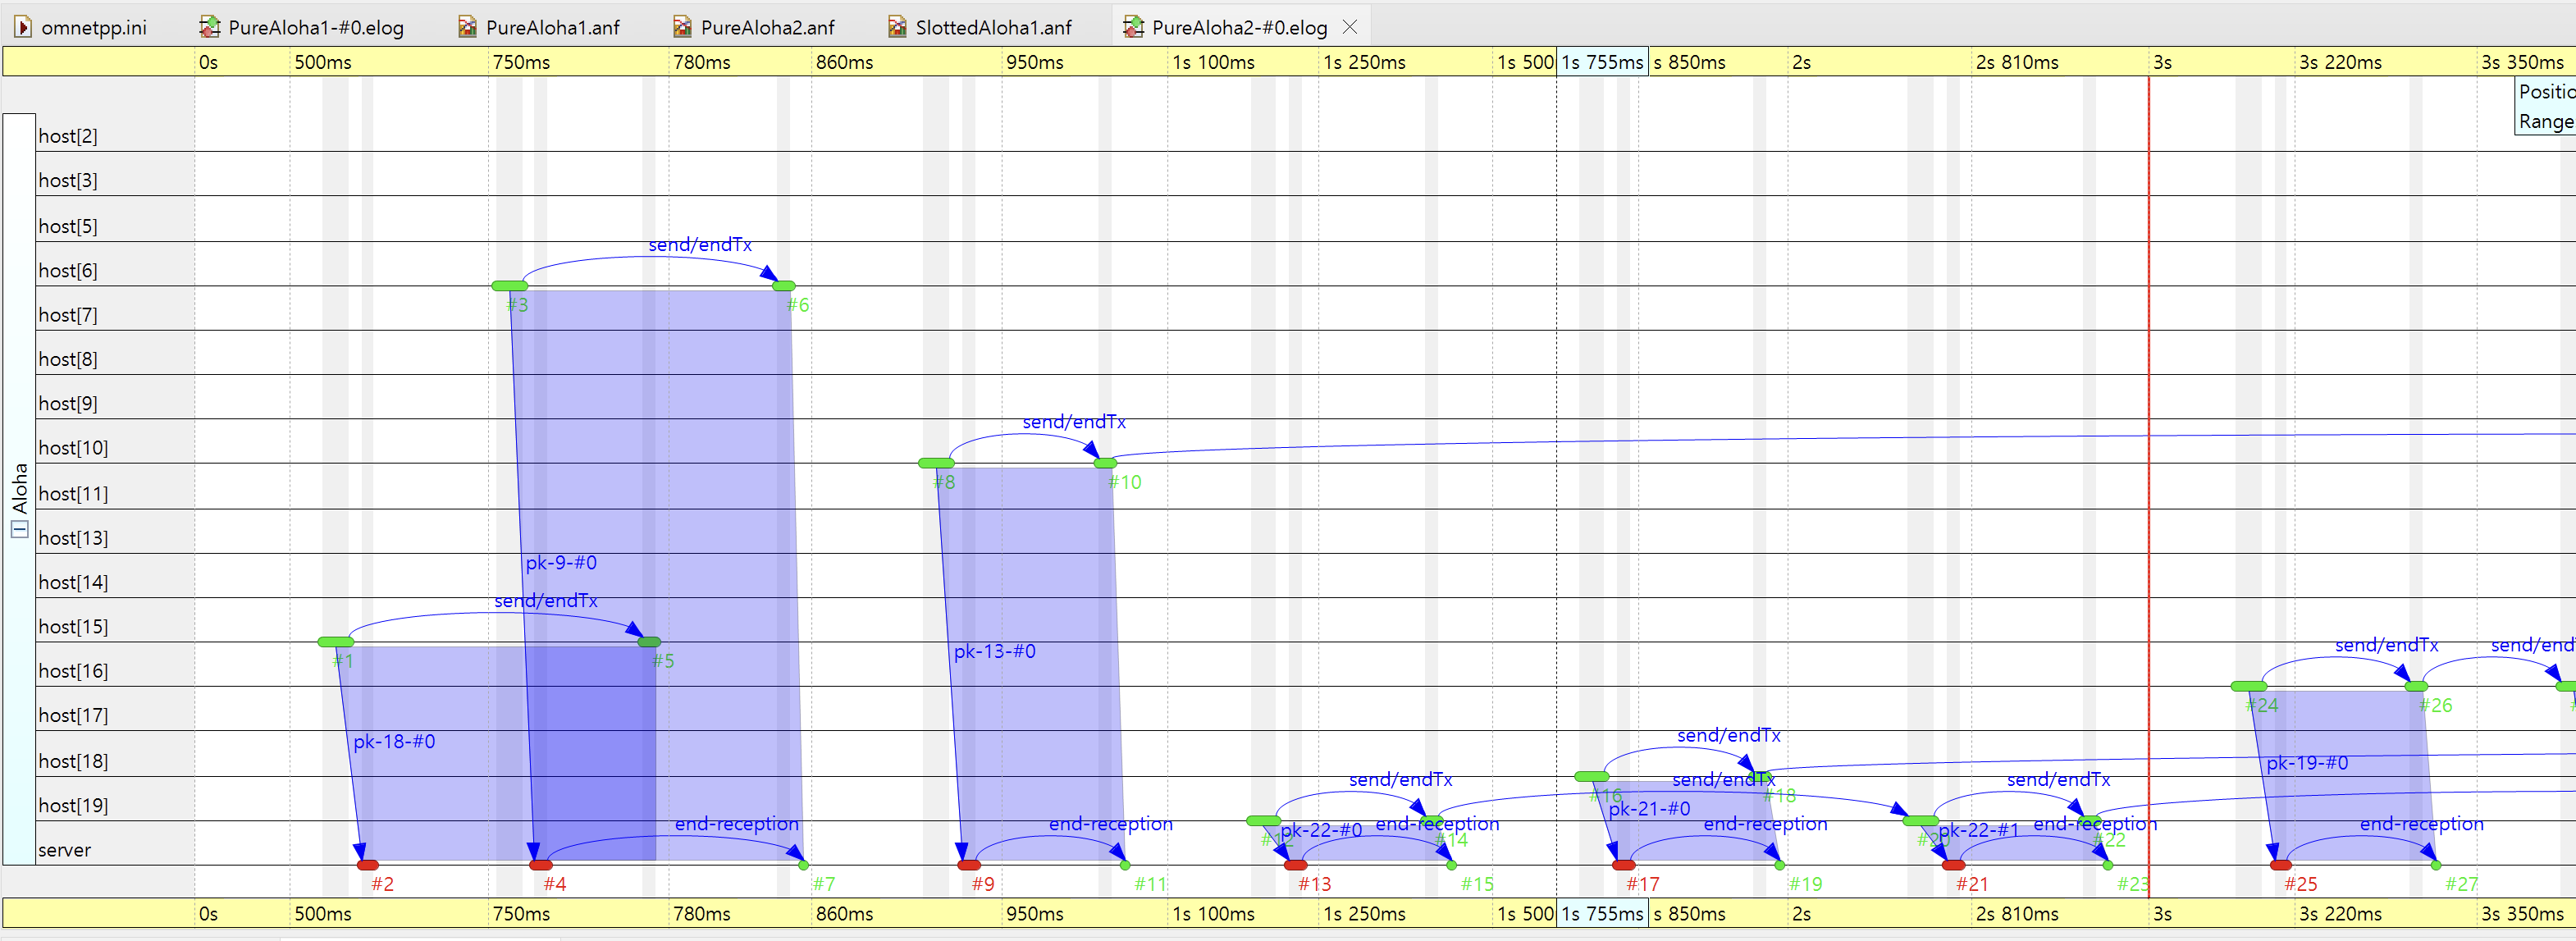
\includegraphics[width=0.93\textwidth]{image/week12/1-1-3.png}
        }\hspace{3mm}
        \subfloat[Slotted Aloha, optimal load]{
            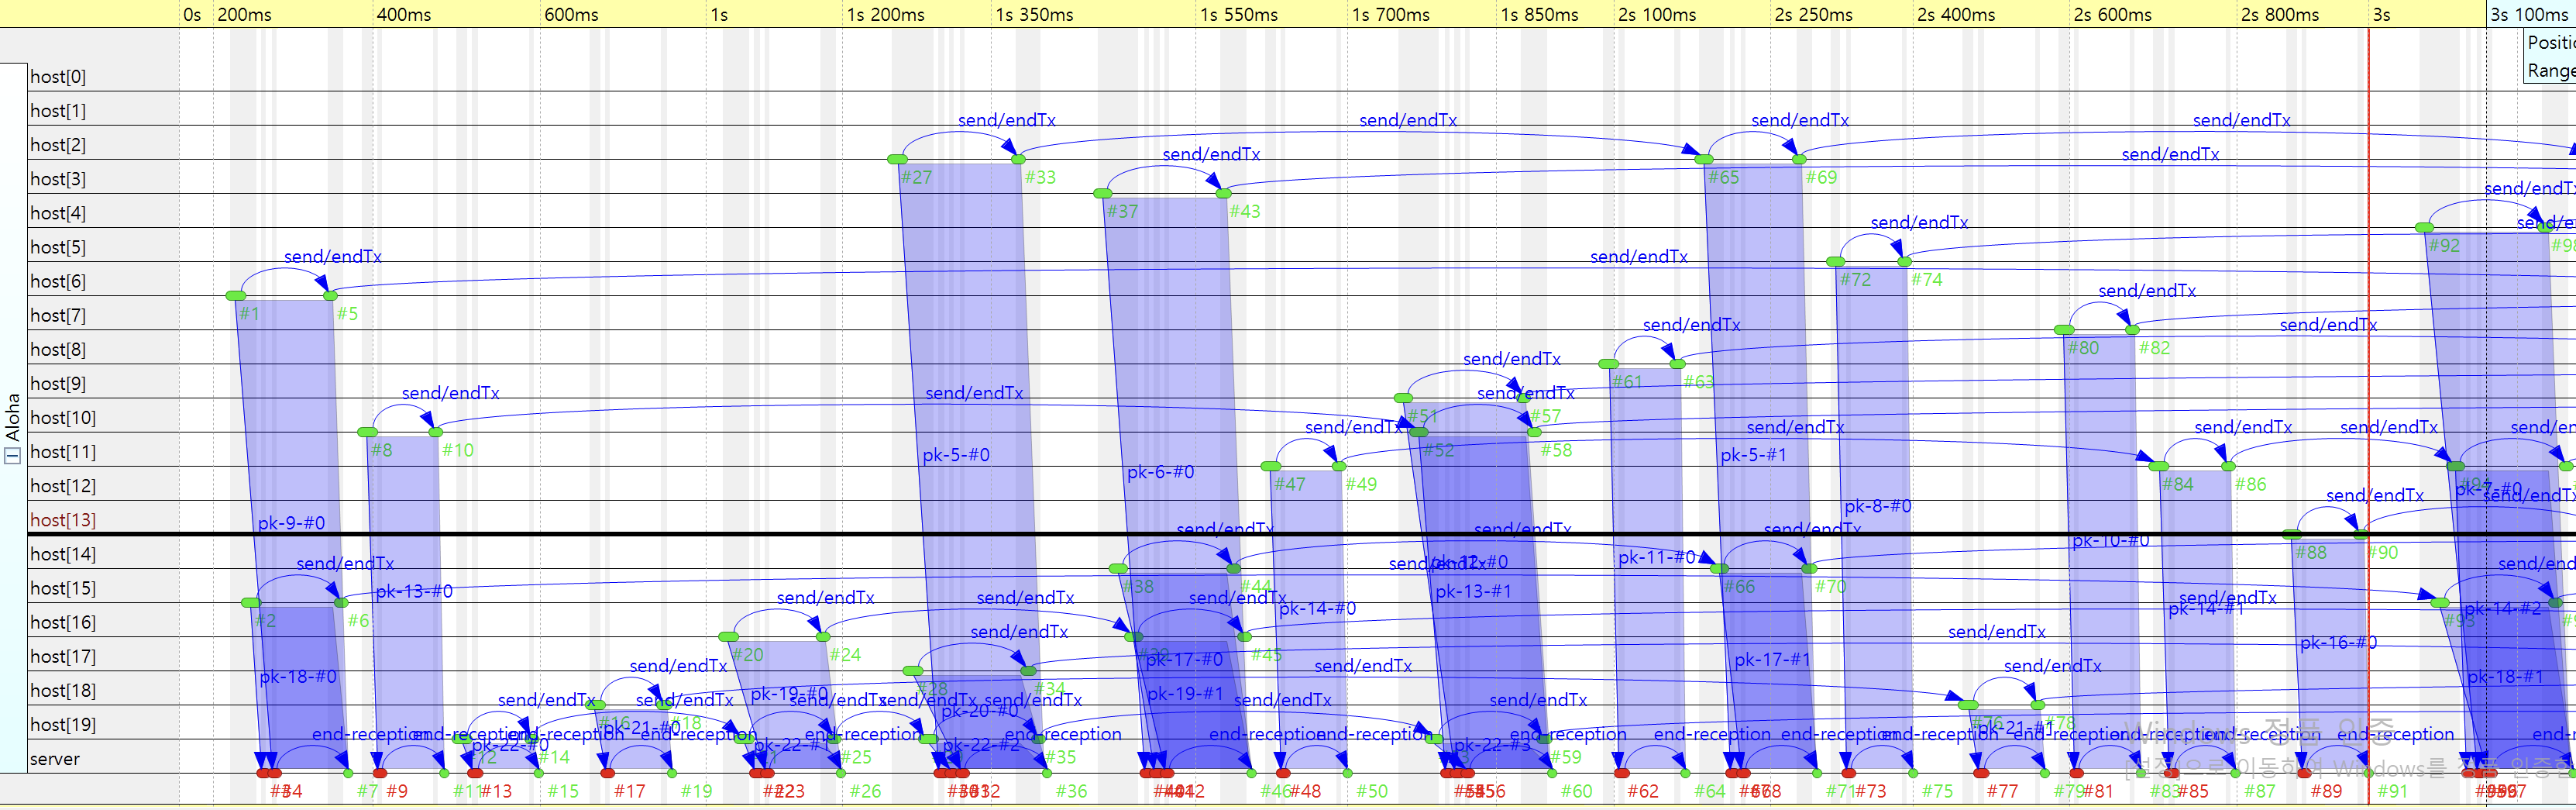
\includegraphics[width=0.93\textwidth]{image/week12/1-1-4.png}
        }
        \vspace{-2mm}
        \caption{Experiment 1-1 Simulation Results Screenshot: Aloha simulation sequence log}
        \end{figure}
     \clearpage
% % 여기서 앞서 정리한 부분의 결과를 확인하는 section 으로 사용한다. -> 다음 
\vspace{-6mm}
\subsection{}
\vspace{-2mm}
\subsubsection{Simulation Results : 채널 효율}
\vspace{-2mm}
    Aloha 와 Slotted aloha를 비교해 주기 위해서 Throughput 을 매개로 G-load 에 따른 비교이기 때문에 Throughput 과 같은 값이라고 할 수 있는 채널효율의 값을 확인해 분석을 하였다.
    Results 에 생성된 sca, 스칼라 파일로부터 aloha server에서 채널 효율값을 확인해 주었다. 
    각각의 scalar 파일을 csv로 변환하여 직접 graph를 그려 분석하려 했으나 \mintinline{c}{scavedata.cc}가 정상적으로 실행되지 않아 sca 에서 직접 확인한 값을 캡처했다.
\vspace{-2mm} 
        \begin{figure}[h!]
        \centering
        \subfloat[Expeitiment 1-1 pure aloha’s Channel Utilizaiton : 0.116946]{
            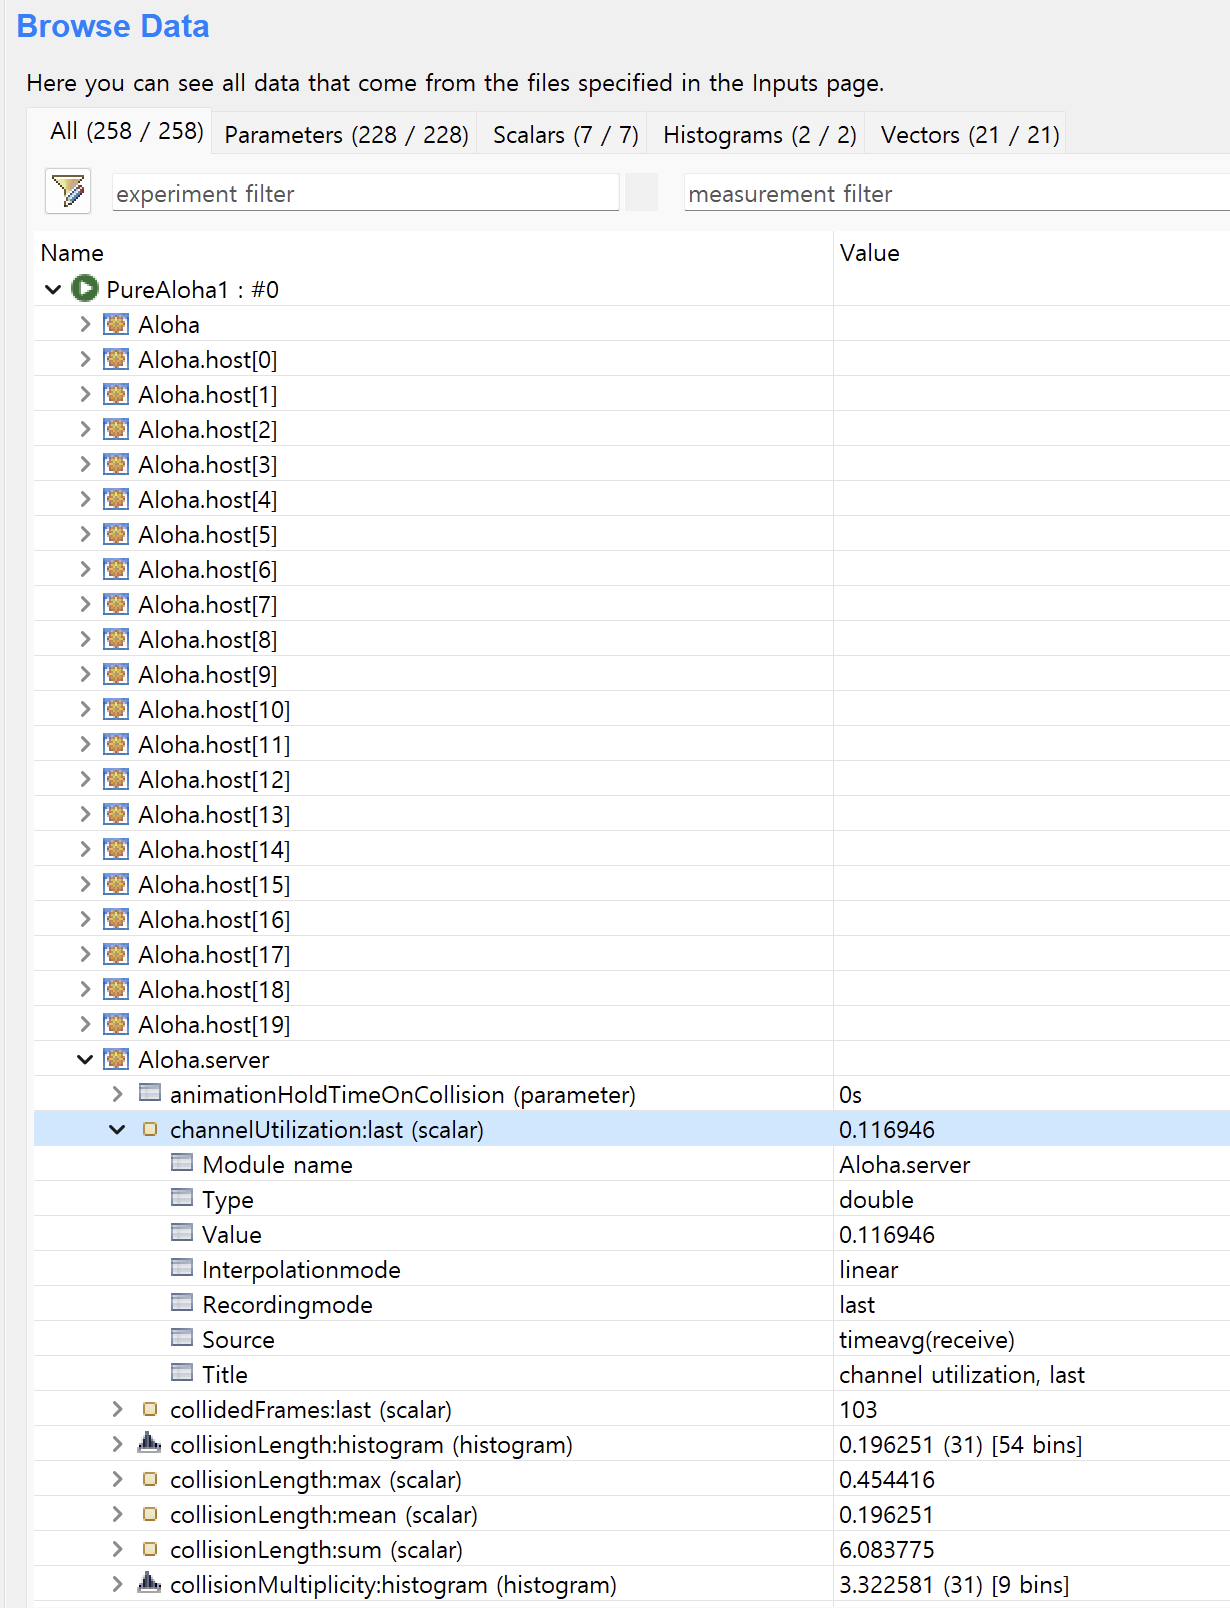
\includegraphics[width=0.43\textwidth]{image/week12/1-2-1.png}
        }\hspace{8mm}
        \subfloat[Expeitiment 1-2 pure aloha’s Channel Utilizaiton : 0.172417]{
            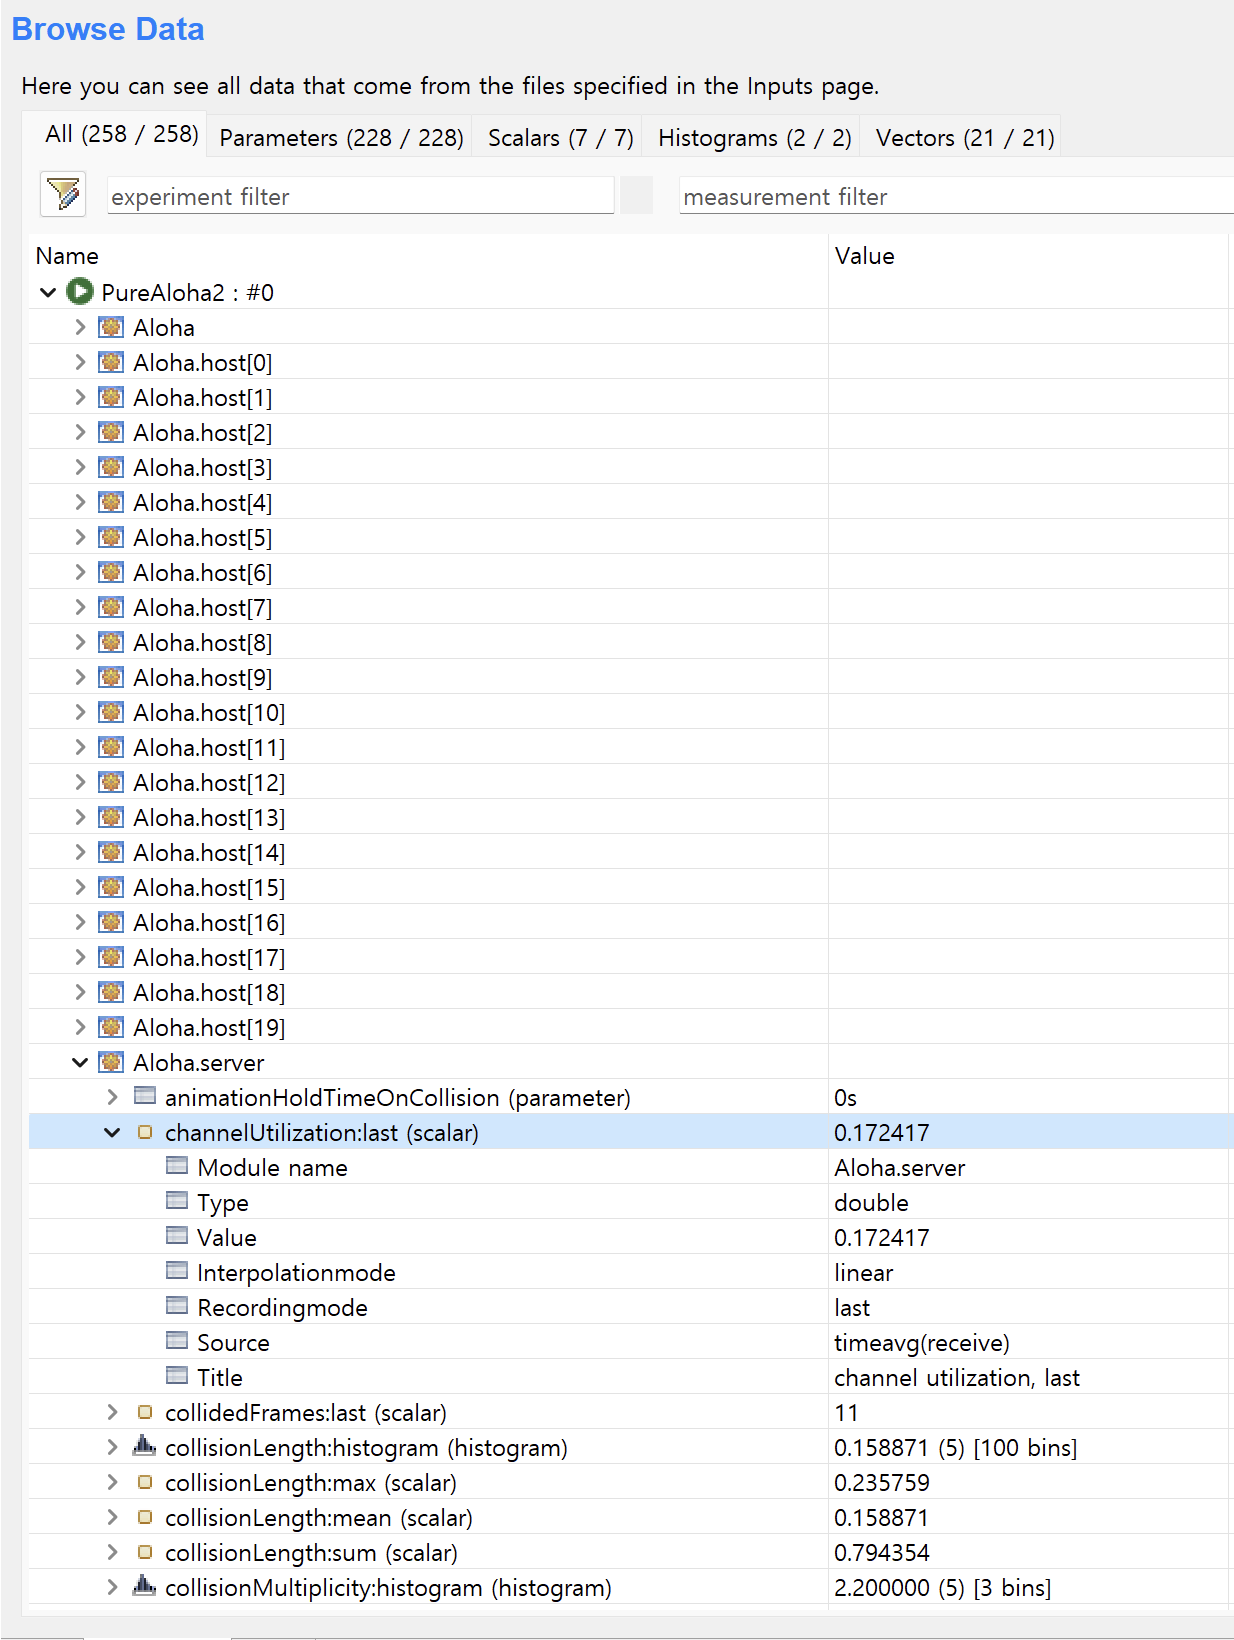
\includegraphics[width=0.43\textwidth]{image/week12/1-2-2.png}
        }\hspace{3mm}
        \subfloat[Expeitiment 1-3 slotted aloha’s Channel Utilizaiton : 0.108012]{
            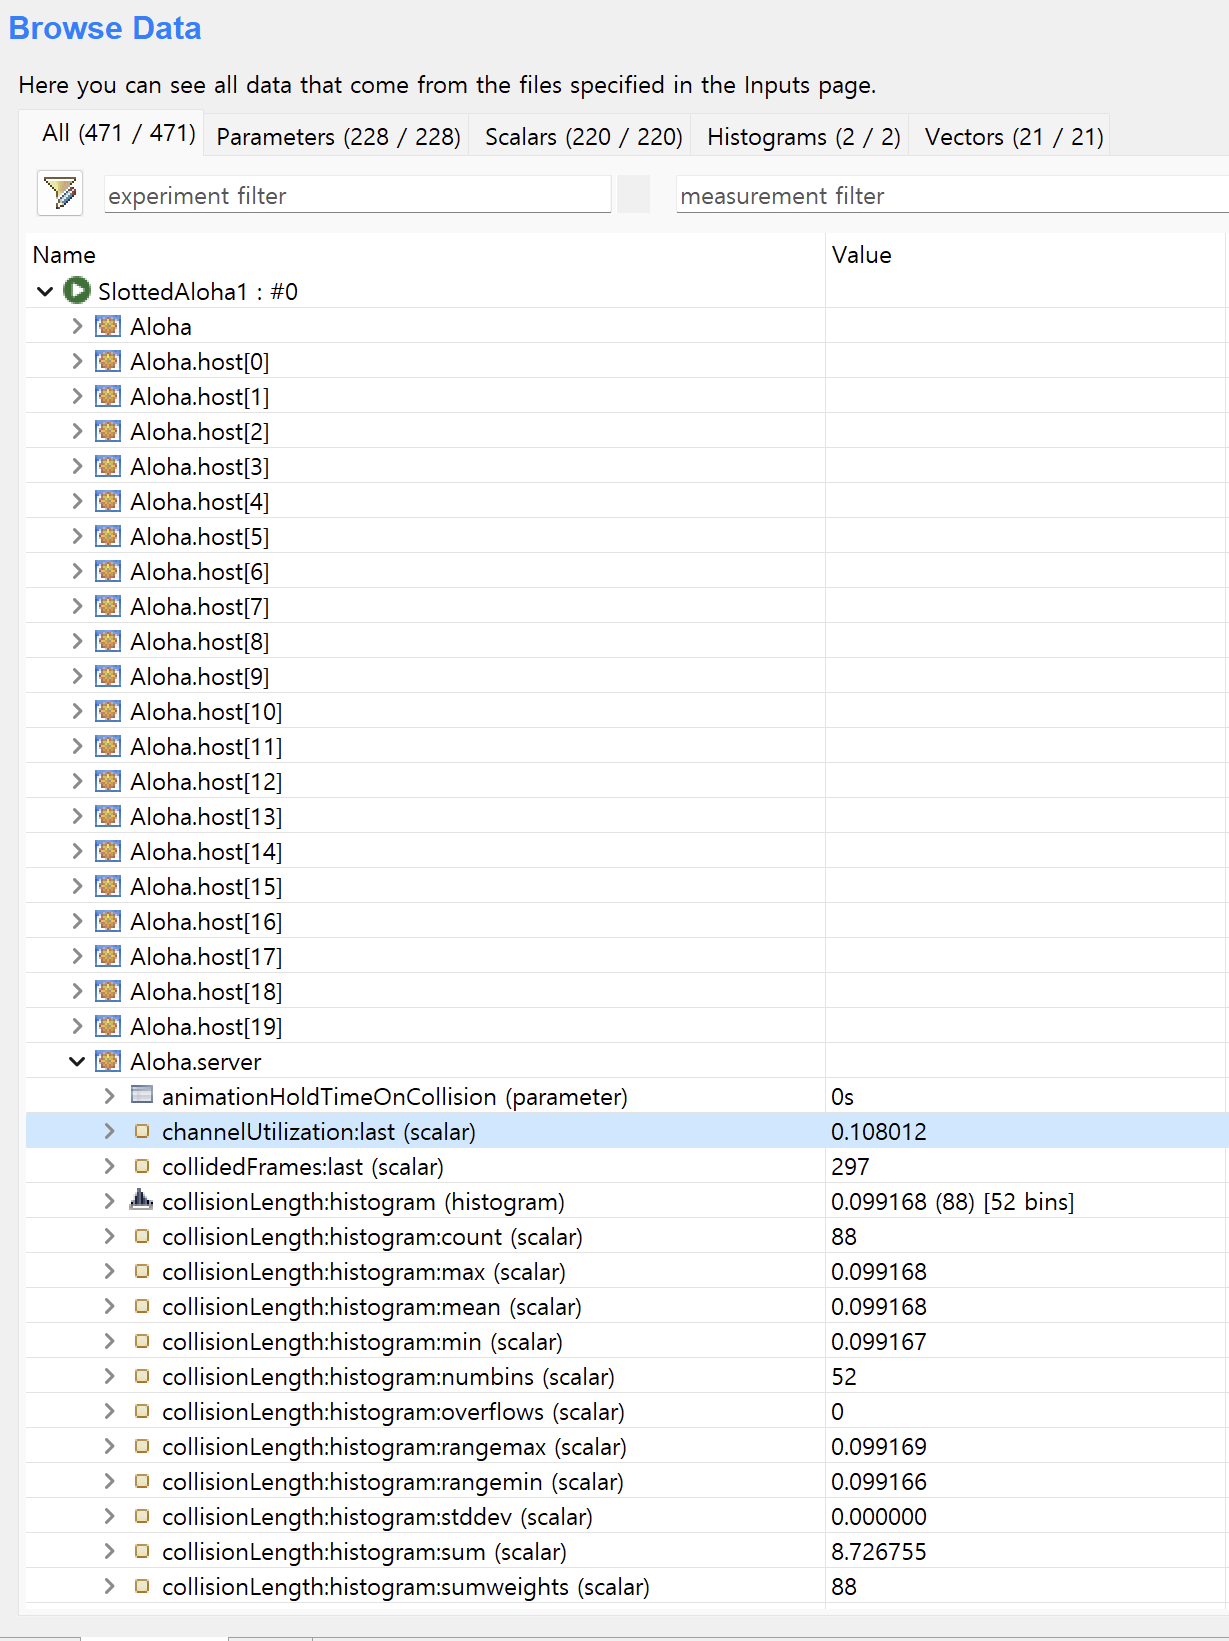
\includegraphics[width=0.43\textwidth]{image/week12/1-2-3.png}
        }\hspace{8mm}
        \subfloat[Expeitiment 1-4 slotted aloha’s Channel Utilizaiton : 0.30498]{
            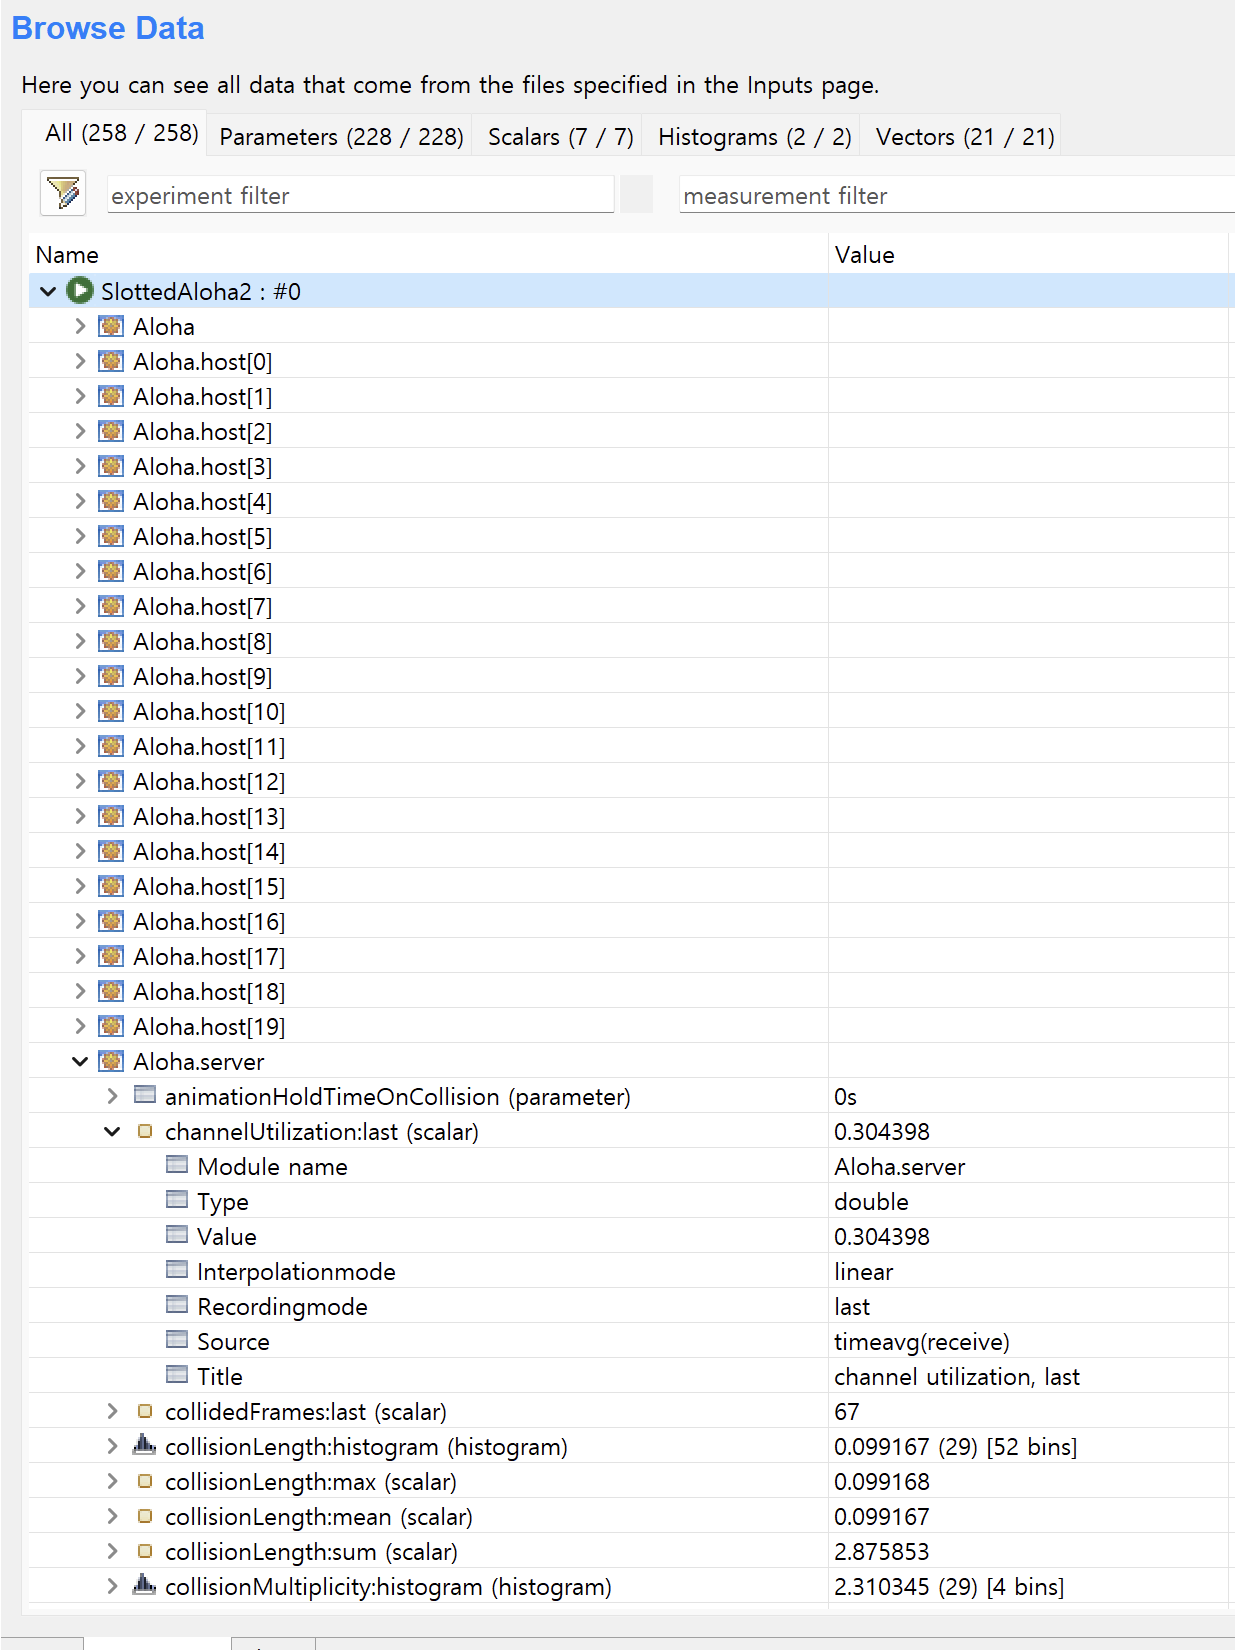
\includegraphics[width=0.43\textwidth]{image/week12/1-2-4.png}
        }
        \vspace{-2mm}
        \caption{Experiment 1-1 Simulation Results Screenshot: packetReceived}
        \end{figure}
    \vspace{-3mm}
\subsubsection{Discussion}
%%------------------------------------------------------------------------------------------
%                                   section intro 2 column
%%------------------------------------------------------------------------------------------
\begin{multicols}{2}
    \begin{minipage}{\columnwidth}
    \vspace{2mm}
    \centering%
    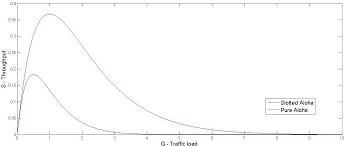
\includegraphics[width=.99\textwidth]{image/week12/1-3.png}
    \vspace{-2mm}
    \captionof{figure}{\small Aloha Throughput Graph depend on G-load}    \vspace{-4mm}
    \end{minipage}
    
    \columnbreak
    
    aloha와 slotted aloha의 차이를 확인하고자 측정한 4가지 조건의 throughput인 채널효율로 부터 pure aloha와 slotted aloha의 각각의 vulnerable time이 2배 차이로 부터 G-load에 상응하는 포아송분포로 표현한 throughput 의 graph와 측정값이 유사하게 나옴으로서 확인했다.
    $$
    S(\text{throughput})= P_{\text{success}} \times G =
    \begin{cases}
    \frac{(2G)^k}{k!}e^{-2G}, & \mbox{pure aloha case}\\
    \frac{(G)^k}{k!}e^{-G}, & \mbox{slotted aloha case}
    \end{cases}
    $$
    \vspace{-4mm}
\end{multicols}
\vspace{-3mm}



% \vspace{-3mm}
\section{}
\vspace{-4mm}
%%------------------------------------------------------------------------------------------
%                                   section intro 2 column
%%------------------------------------------------------------------------------------------
\begin{multicols}{2}
    \begin{minipage}{\columnwidth}
    \vspace{2mm}
    \centering%
    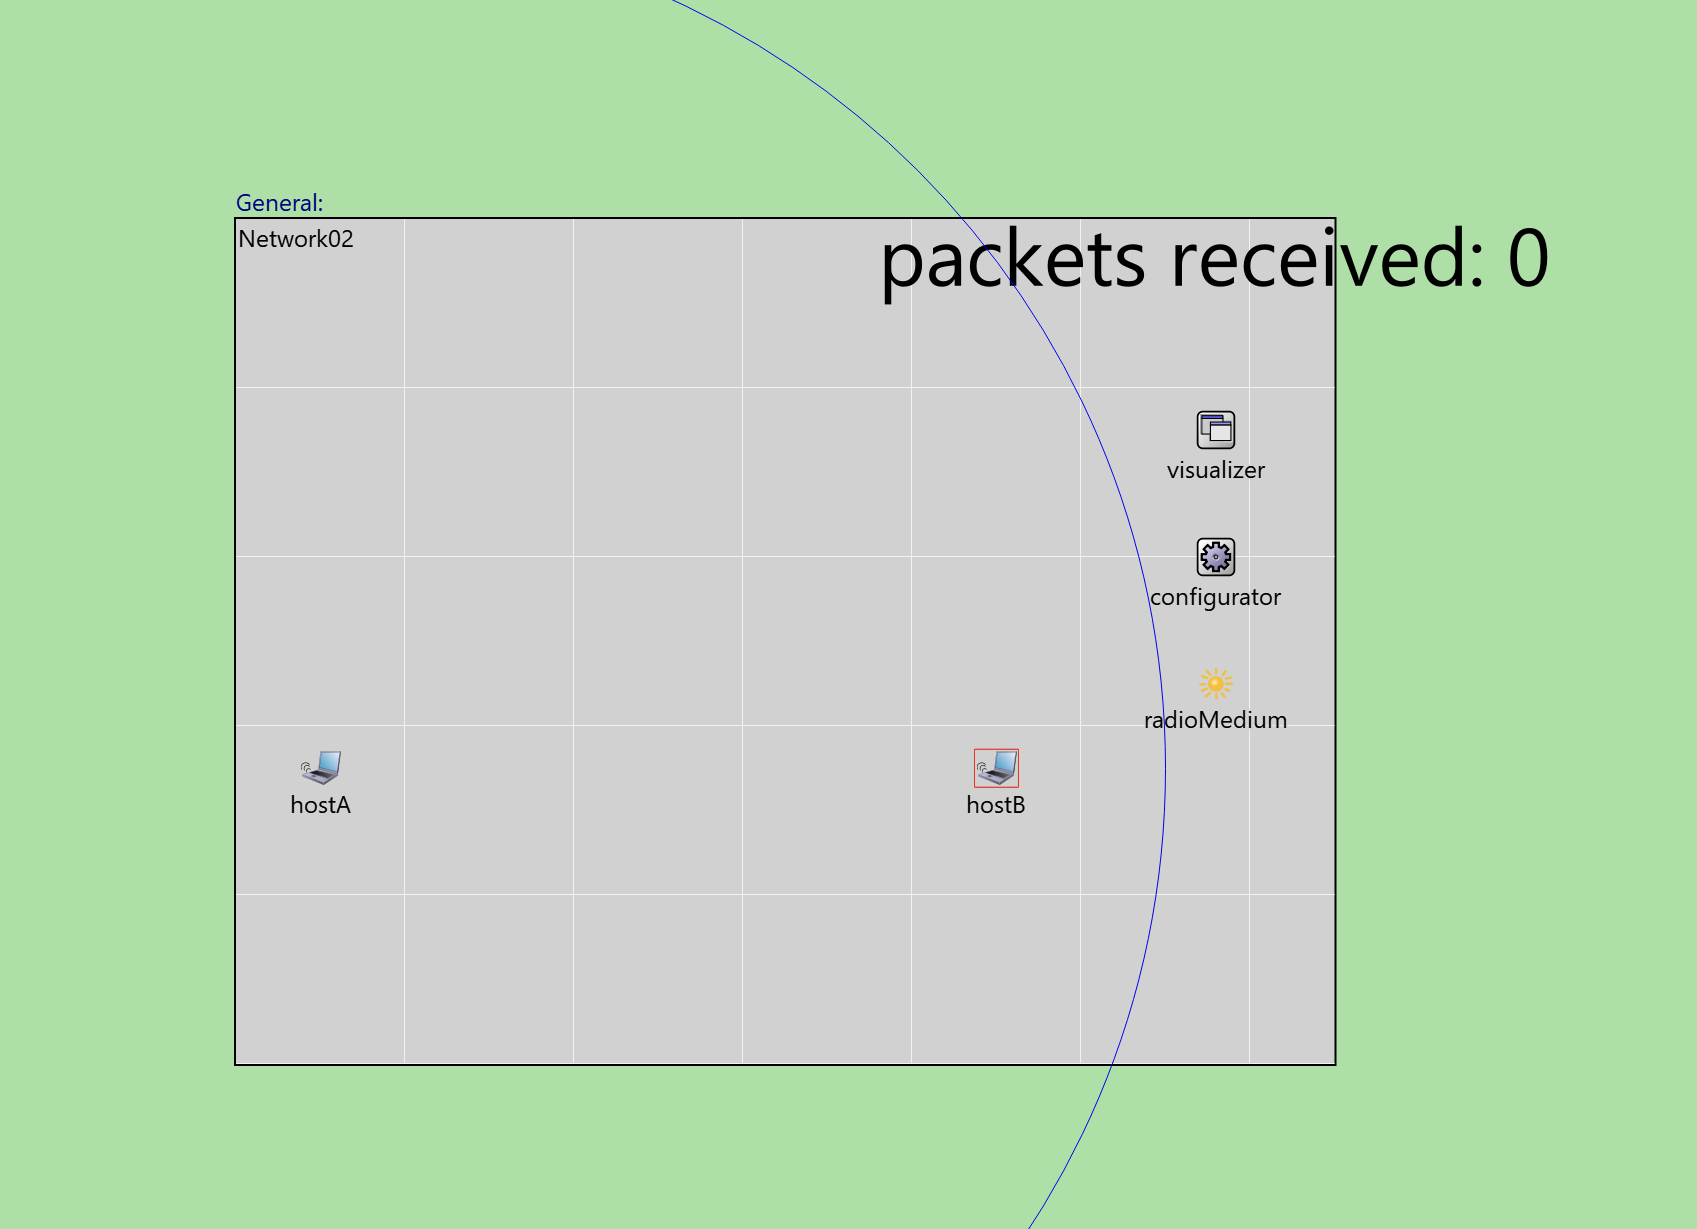
\includegraphics[width=.9\textwidth]{image/week12/2-1.png}
    \vspace{-2mm}
    \captionof{figure}{\small Hidden Node Problem Diagram}    \vspace{-4mm}
    \end{minipage}
    
    \columnbreak
    
    Experiment 2,3,4 에서는 INET framework 에서 무선 시뮬리에션을 구축해 본다.
    
    Experiment 2 에서는 무선으로 통신하는 2 HOST의 simulation 실험으로,  한 HOST가 다른 HOST에게 UDP 데이터 스트림을 무선으로 보내는 네트워크를  구성한다.
    HOST A가 1000 byte 크기의 UDP packet을 생성하여 HOST B 에게 평균 10ms의exponential distribution을 가지는 무작위 간격으로 전송한다.
    이때 2개의 host의 간격은 400m로, ini 에서 설정해준 network의 유효 통신범위radio.transmitter.communicationRange 의 500m 이내이므로 직접 통신이 가능한 기본적인 네트워크에서 simulation을 진행한다.
    \vspace{-4mm}
\end{multicols}
\vspace{-4mm}
%%%%%%%%%%%%%%%%%%%%%%%%%%%%%%%%%%%%%%%%%%%%%%%%%%%%%%%%%%%%%%%%%%%%%%%%%%%%%%%%%%%%%%%%%%%%
%%------------------------------------------------------------------------------------------
%                                   Cose Reference
%%------------------------------------------------------------------------------------------
\vspace{-4mm}
\subsection*{CODE}
\vspace{-3mm}
lecture 에서 blank를 채운 코드이외에 lecrure에서 주어진 실행 code들은 보고서 마지막 appendix에 첨부했다.
\vspace{-3mm}
    \subsubsection*{Network02.ompnetpp.ini}
        \vspace{-2mm}
        \begin{listing}[h!]
        \inputminted[framerule = 1pt,framesep = 2mm , frame = lines, fontsize=\scriptsize]{c}{./code/week12/Experiment_02/ini.cpp}
        \vspace{-3mm}
        \caption{\footnotesize Network02.ned}
        \vspace{-3mm}
        \end{listing}
        \vspace{-6mm}
\clearpage
%%%%%%%%%%%%%%%%%%%%%%%%%%%%%%%%%%%%%%%%%%%%%%%%%%%%%%%%%%%%%%%%%%%%%%%%%%%%%%%%%%%%%%%%%%%%
%%------------------------------------------------------------------------------------------
%           simulation results -> you tube 링크 + 스크린샷 2장 + 내용에 대한 설명
%%------------------------------------------------------------------------------------------
\subsection*{SIMULATION RESULTS}
    \vspace{-1mm}
    Host A 에서 Host B로 UDP packet을 전송하는 동작을 네트워크 외부, Host A 내부, Host B 내부 동작의 화면녹화 영상을 업로드하였다.
    simulation 전체의 영상은 아래 링크를 클릭하여 확인할 수 있다.     
    \vspace{-10mm}
        \begin{center}
            \item \href{https://youtu.be/N8wHft9a8jM}
        	{Youtube link of Week12 Experiment 02 Simulation Results Screenshot Video}
        \end{center}
    \vspace{-6mm}
    % 사진 1 2개는 넣어 주자
        \begin{figure}[h!]
        \centering
        \subfloat{
            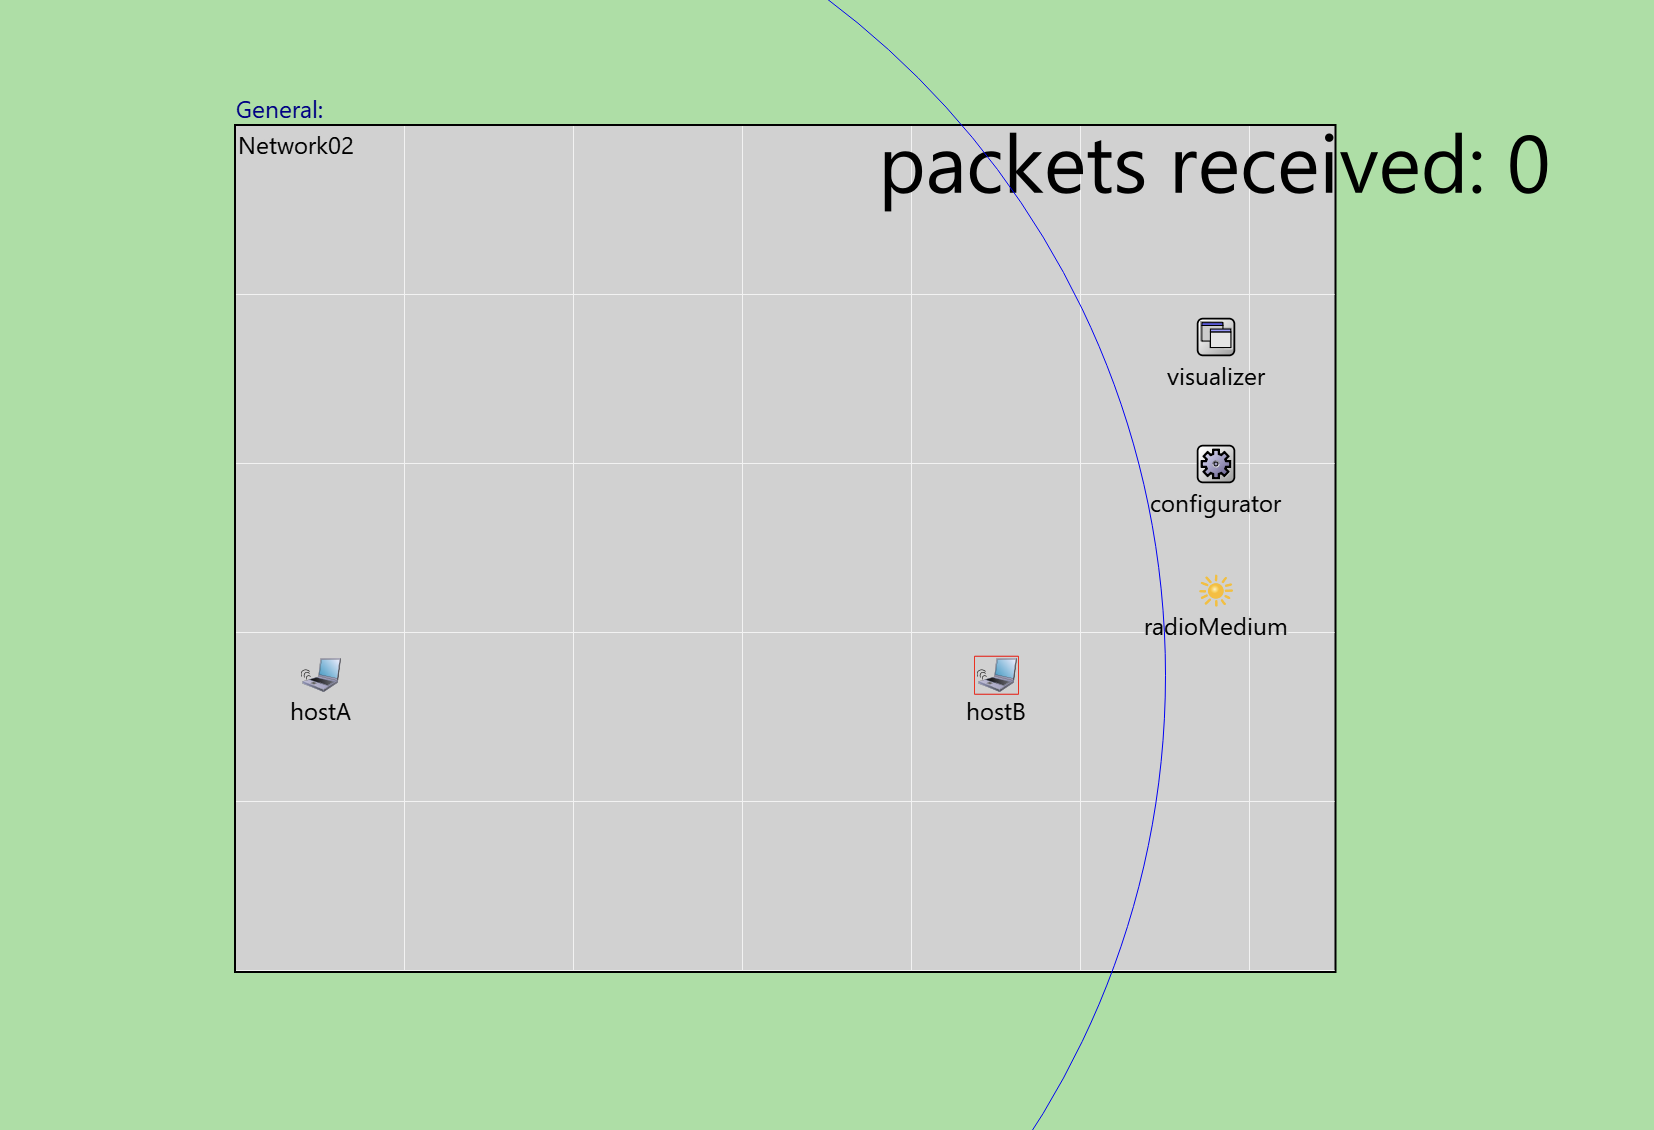
\includegraphics[width=0.46\textwidth]{image/week12/2-2-1.png}
        }\hspace{3mm}
        \subfloat{
            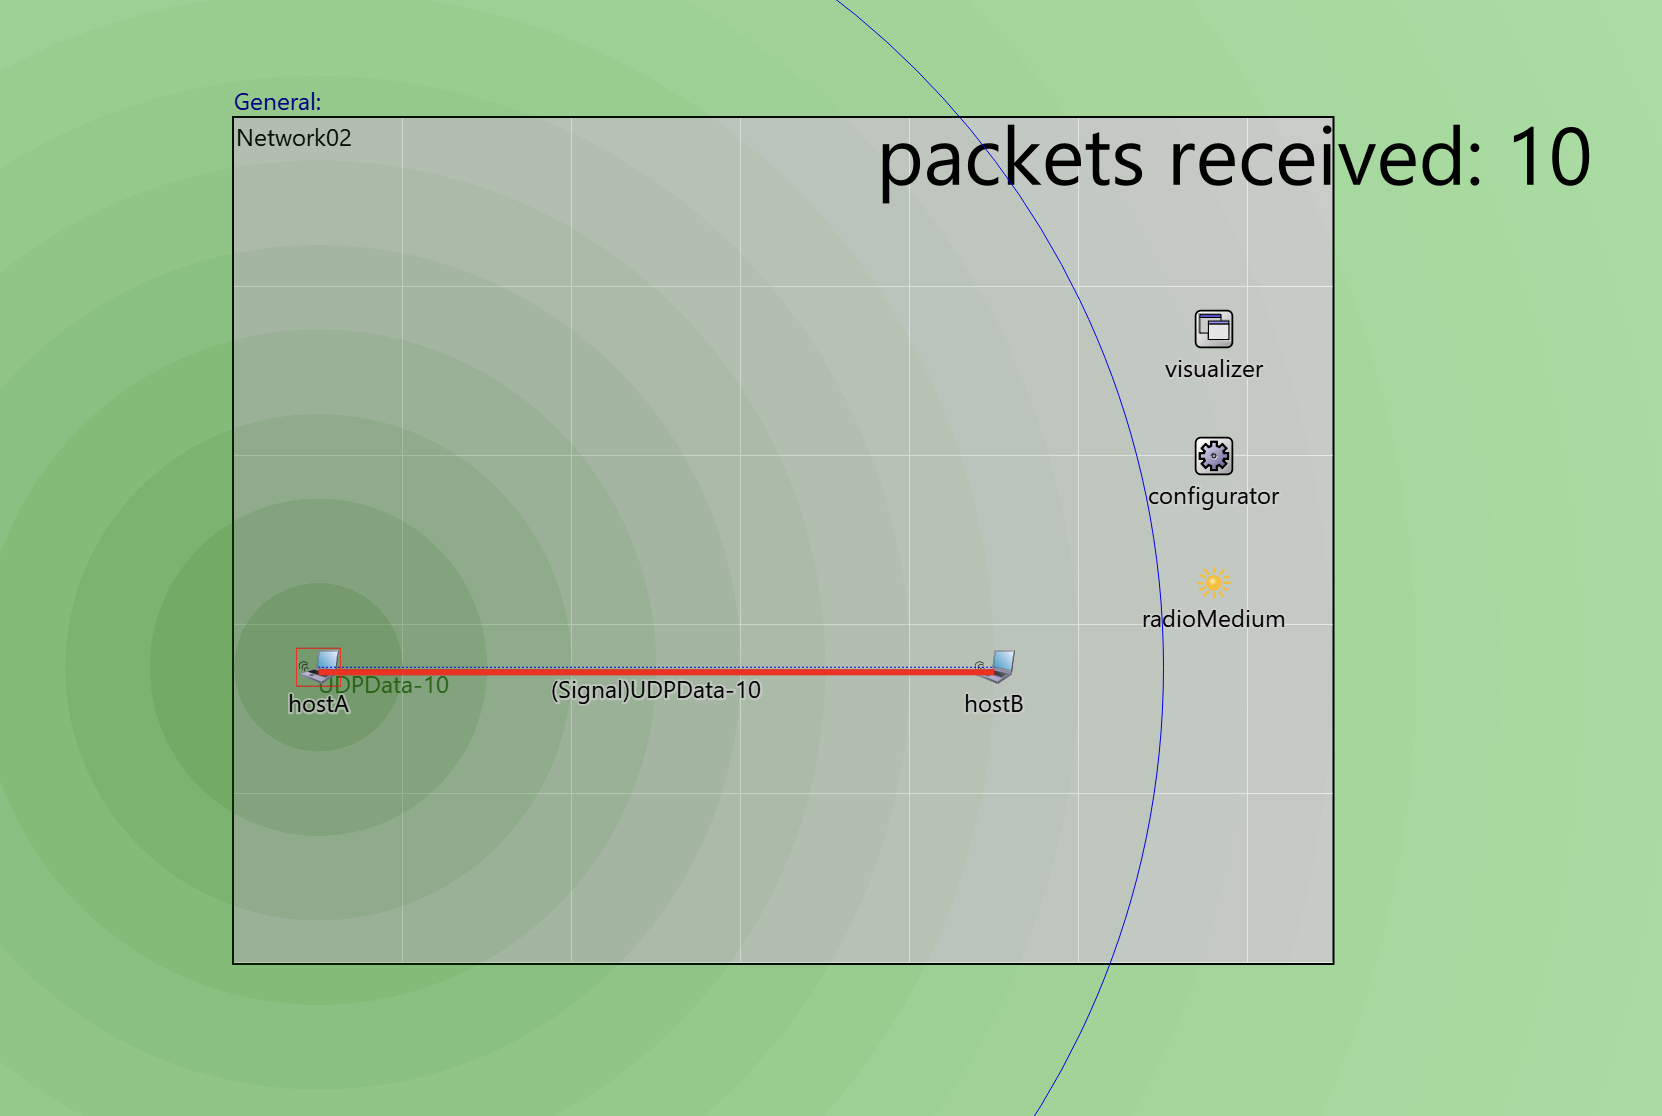
\includegraphics[width=0.46\textwidth]{image/week12/2-2-2.png}
        }
        \caption{Experiment 02 Simulation Results Screenshot}
        \vspace{-2mm}
        \end{figure}
    
    simulation 의 flow는 다음과 같다. 
\vspace{-3mm}
    \subsubsection*{Transfer Model }
    \vspace{-2mm}
    Host A 가 Host B에게 전송하는 10ms 의 exponential 한 분포를 따르는 무작위 간격으로 1000 바이트 크기의 UDP 트래픽을 생성해 전송한다.  그리고 ini 에 추가해준 visulaize함수로 Host B 가 받은 패킷수를 표기해 주었다. 
\vspace{-1mm}
    \subsubsection*{Physical Layer Modelling }
    \vspace{-2mm}
    ini 에서 가능한 무선 통신 연결거리를 500m, 1Mbps의 속도로 데이터가 전송이되고, ned 에서 Host A 와 Host B의 간격을 450m 로 설정해주어 직접 통신이 가능하도록 설정해 주었다. 
    \subsubsection*{Simulation Scenario}
    Host A 에서 임의의 간격으로 UDP pacjet을 생성해주고, 생성된 packet은 IPv4 를 통해서네트워크 later로 이동한다. 이때 네트워크 layer에서 packet은 전송 대기열이 진행하는 simulation처럼 없으면 바로 전송이 이뤄진다. 이후 Host A 에서 Host B로 바로 모든 packet이 전송된다.
    
\clearpage
% \vspace{-3mm}
\section{}
%%------------------------------------------------------------------------------------------
%                                   Cose Reference
%%------------------------------------------------------------------------------------------
\vspace{-4mm}
\subsection*{CODE}
\vspace{-3mm}
Experiment 3에서는 routing을 하는 3개의 host를 추가한다.  추가하는 host에서 IPv4 static routing 을 통해서 Host A 에서 Host B 로 packet이 전송될 수 있도록해준다. Host R1 R2 R3 를 추가해주는 코드로, 기존의  에서 extends를 이용하여   를 설정해 주었고, initial  file에서 IPv4 forward routing의 코드를 추가해 준다.
    \vspace{-3mm}
\subsubsection*{Experiment03.ini}
    \vspace{-2mm}
    \begin{listing}[h!]
    \inputminted[framerule = 1pt,framesep = 2mm , frame = lines, fontsize=\footnotesize ]{c}{./code/week12/Experiment_03/ini.cpp}
    \vspace{-3mm}
    \caption{\footnotesize Expeirment 03's ini file, add forward routing}
    \end{listing}
    \vspace{-6mm}
\subsubsection*{Network.ned}
    \vspace{-2mm}
    \begin{listing}[h!]
    \inputminted[framerule = 1pt,framesep = 2mm , frame = lines, fontsize=\footnotesize ]{c}{./code/week12/Experiment_03/Network03.cpp}
    \vspace{-3mm}
    \caption{\footnotesize Expeirment 03's network file, add three of routing host}
    \end{listing}
    \vspace{-6mm} 
    
%%%%%%%%%%%%%%%%%%%%%%%%%%%%%%%%%%%%%%%%%%%%%%%%%%%%%%%%%%%%%%%%%%%%%%%%%%%%%%%%%%%%%%%%%%%%
%%------------------------------------------------------------------------------------------
%           simulation results -> you tube 링크 + 스크린샷 2장 + 내용에 대한 설명
%%------------------------------------------------------------------------------------------
\subsection*{SIMULATION RESULTS}
    Experiment 3에서는 routing을 하는 3개의 host를 추가한다. 이때 routing에 의미가 있기위해 Host A와 Host B의 유효 거리를 500 m 에서 250m 로 줄여주어 직접적인 전송이 되지 않도록 변경해 주었다. 
    simulation 전체의 영상은 아래 링크를 클릭하여 확인할 수 있다.     
    \vspace{-10mm}
        \begin{center}
            \item \href{https://www.youtube.com/watch?v=WlI24BkZjFs&ab_channel=anamnesis}
        	{Youtube link of Week12 Experiment 03 Simulation Results Screenshot Video}
        \end{center}
    \vspace{-6mm}
    % 사진 1 2개는 넣어 주자
        
\vspace{-3mm}
    \subsubsection*{Physical Layer Modelling}
    \vspace{-2mm}
    ini 에서 가능한 무선 통신 연결거리를 250m, 1Mbps의 속도로 데이터가 전송이되고, ned 에서 Host A 와 Host B의 간격을 450m 로 설정해주어 직접 통신이 불가능하고 Host R1의 routing 을 통해서 전송이 되도록 구성해 주었다. 
    \subsubsection*{Simulation Scenario}
    \vspace{-2mm}
    Experiment 2 에서의 Host A 와 Host B 사이에서 직접 무선연결에서 유효 통신거리를 250 m로 줄여줌으로서 새로 추가해준 Host R1을 통한 정적 라우팅을 확인한다. 이는 pre report 에서 다룬 hidden node problem 에 해당되는 네트워크 시나리오 임을 알 수 있다. 
    업로드 한 영상은 전체 네트워크에서의 네트워크의 흐름과 host b 내부에서 어떻게 packet을 받는지의 동작을 캡처했다. 
    전체 네트워크에서 host A에서 host B로 패킷을 전송하지만 이는 링크에서 폐기되는 유효한 부분이 아니다. 이때의 routing 의 동작은 sequence log의 info 에서 확인할 수 있는것과 같이 정적 라우팅 테이블에 따라서 진행됨을 확인할 수 있다. 
    Routing 과정에서 router역할을 하는 host들은 half parent 이므로 동시에 송수신이 불가능하기때문에 결과적으로 host a에서 전송한 udp 프레임의 절반만이 host b로 전송되는 일종의 서로를 인지 못한 두 호스트 사이에서의 송수신이 충돌해 효율이 감소하는 hidden node problem이 야기되는 결과 또한 확인이 가능하다.

% \vspace{-3mm}
\section{}
%%------------------------------------------------------------------------------------------
%                                   Cose Reference
%%------------------------------------------------------------------------------------------
\vspace{-4mm}
\subsection*{CODE}
\vspace{-3mm}
Experimnet 3의 동일한 network에서 CSMA 를위한 condition을 추가한다. 뿐만 아니라 조금더 복잡한 네트워크 환경을 simulation 해주기 위해서 inference range의 설정을 통해서 host a와 host b 사이에서 전송을 할 수 없지만 이에 따른 간섭의 영향을 추가한다.
사용하는 csma protocol에 ack응답을 추가해주어 신뢰성을 높인 네트워크를 simulation 한다.
\vspace{-3mm}
\subsubsection*{Experiment04.ini}
    \vspace{-2mm}
    \begin{listing}[h!]
    \inputminted[framerule = 1pt,framesep = 2mm , frame = lines, fontsize=\footnotesize ]{c}{./code/week12/Experiment_04/ini.cpp}
    \vspace{-3mm}
    \caption{\footnotesize Expeirment 03's ini file, using csma/ca as MAC with ACK}
    \end{listing}
    \vspace{-6mm} 
%%%%%%%%%%%%%%%%%%%%%%%%%%%%%%%%%%%%%%%%%%%%%%%%%%%%%%%%%%%%%%%%%%%%%%%%%%%%%%%%%%%%%%%%%%%%
%%------------------------------------------------------------------------------------------
%           simulation results -> you tube 링크 + 스크린샷 2장 + 내용에 대한 설명
%%------------------------------------------------------------------------------------------
\subsection*{SIMULATION RESULTS}
    simulation 전체의 영상은 아래 링크를 클릭하여 확인할 수 있다.     
    \vspace{-10mm}
        \begin{center}
            \item \href{https://www.youtube.com/watch?v=WlI24BkZjFs&ab_channel=anamnesis}
        	{Youtube link of Week12 Experiment 04 Simulation Results Screenshot Video}
        \end{center}
    \vspace{-6mm}
    % 사진 1 2개는 넣어 주자
         
\vspace{-3mm}
    \subsubsection*{Physical Layer Modelling  }
    \vspace{-2mm}
    ini 에서 가능한 무선 통신 연결거리를 500m, 1Mbps의 속도로 데이터가 전송이되고, ned 에서 Host A 와 Host B의 간격을 450m 로 설정해주어 직접 통신이 가능하도록 설정해 주었다. 
\vspace{-1mm}
    \subsubsection*{Simulation Scenario }
    \vspace{-2mm}
    앞선 experiment 1,2의 MAC  protocol들은 채널상에 올라온 패킷들을 즉시 전송하여 collision이 구조적으로 높게 발생하였다. 
    CSMA /CA는 다른 노드들의 전송상태를 채크함으로서 충돌을 회피한다. 여기에 ACK 을 사용하여 다른 노드들에게 채널이 비어있음을 알린다.
    Host A 에서 임의의 간격으로 UDP packet을 생성해주고, 생성된 packet은 IPv4 를 통해서네트워크 later로 이동한다. 이때 네트워크 layer에서 packet은 전송 대기열이 진행하는 simulation처럼 없으면 바로 전송이 이뤄진다. 이후 Host A 에서 Host B로 바로 모든 packet이 전송된다. 
\section*{Discussion}
\vspace{-3mm}
실험 2,3 그리고 4를 진행하면서 네트워크의 변화는 다음과 같다. 
\vspace{-3mm}
    \subsubsection*{EX02 $\rightarrow$ EX03}
\vspace{-2mm}
Routing host를 추가하고 Host A와 Host B사이의 통신이 Host R1을 통해서 이루어지게 된다.
Hidden Node Problem으로, 전송되는 UDP packet을 확인해 보았을때 NIC 에서 각 NODE들은 언제나 수신하거나 송신할 수 있지만 동시에 진행이 되지 못하기 떄문에 실질적으로 전송되는 PACKET의 수는 실험 3에서 실험 2와 비교해 보았을때 절반정도만 전송이 되는 결과를 확인할 수 있었다. 
\vspace{-3mm}
    \subsubsection*{EX03 $\rightarrow$ EX04}
\vspace{-2mm}
실험 3의 network 에서 ACK을 사용하는 CSMA / CA를 MAC으로 사용한다. 추가로 ACK의 사용여부에 따른 차이를 확인하기 위해서 ini 파일에서 \mintinline{c}{host*.wlan[0].mac.useAck = false}로 설정해준 일반 CSMA의 실험을 진행해 주어 결과를 비교해 보았다. Figure 6 (a)에서 UDP-Packet 0 가 전송되는 과정을 보면, Host R1 에서 Host B로 back off timer가 지난후 바로 전송이 이루어짐을 확인할 수 있다. 이 과정에서의 소요시간을 실험 2 와 비교해 보면 대략적으로 7배 빠른 CSMA 의 이점을 확인할 수 있다. 

Figure 6 (b) 에서는 추가적으로 ACK을 사용함으로서, Host R1 에서 Host B 로  UDP-Packet 0을 전송할때 확산시키는 CsmaAck을 수신받아야 UDP packet을 전송하는 과정으로 실험3에서 일정시간 후 전송에서 변화된점을 확인할 수 있다. 이를 통해서 ACK이 없는경우에 비해 손실된 packet이 거의 없이 안정적으로 데이터를 전송할 수 있지만, 만일 네트워크가 혼잡한 경우 collision에 따라서 ACK의 수신에 따른 delay가 심화될 수 있는 단점 또한 확인할 수 있다.\\
\begin{figure}[h!]
\centering
\subfloat[Experiment04 csma ]{
    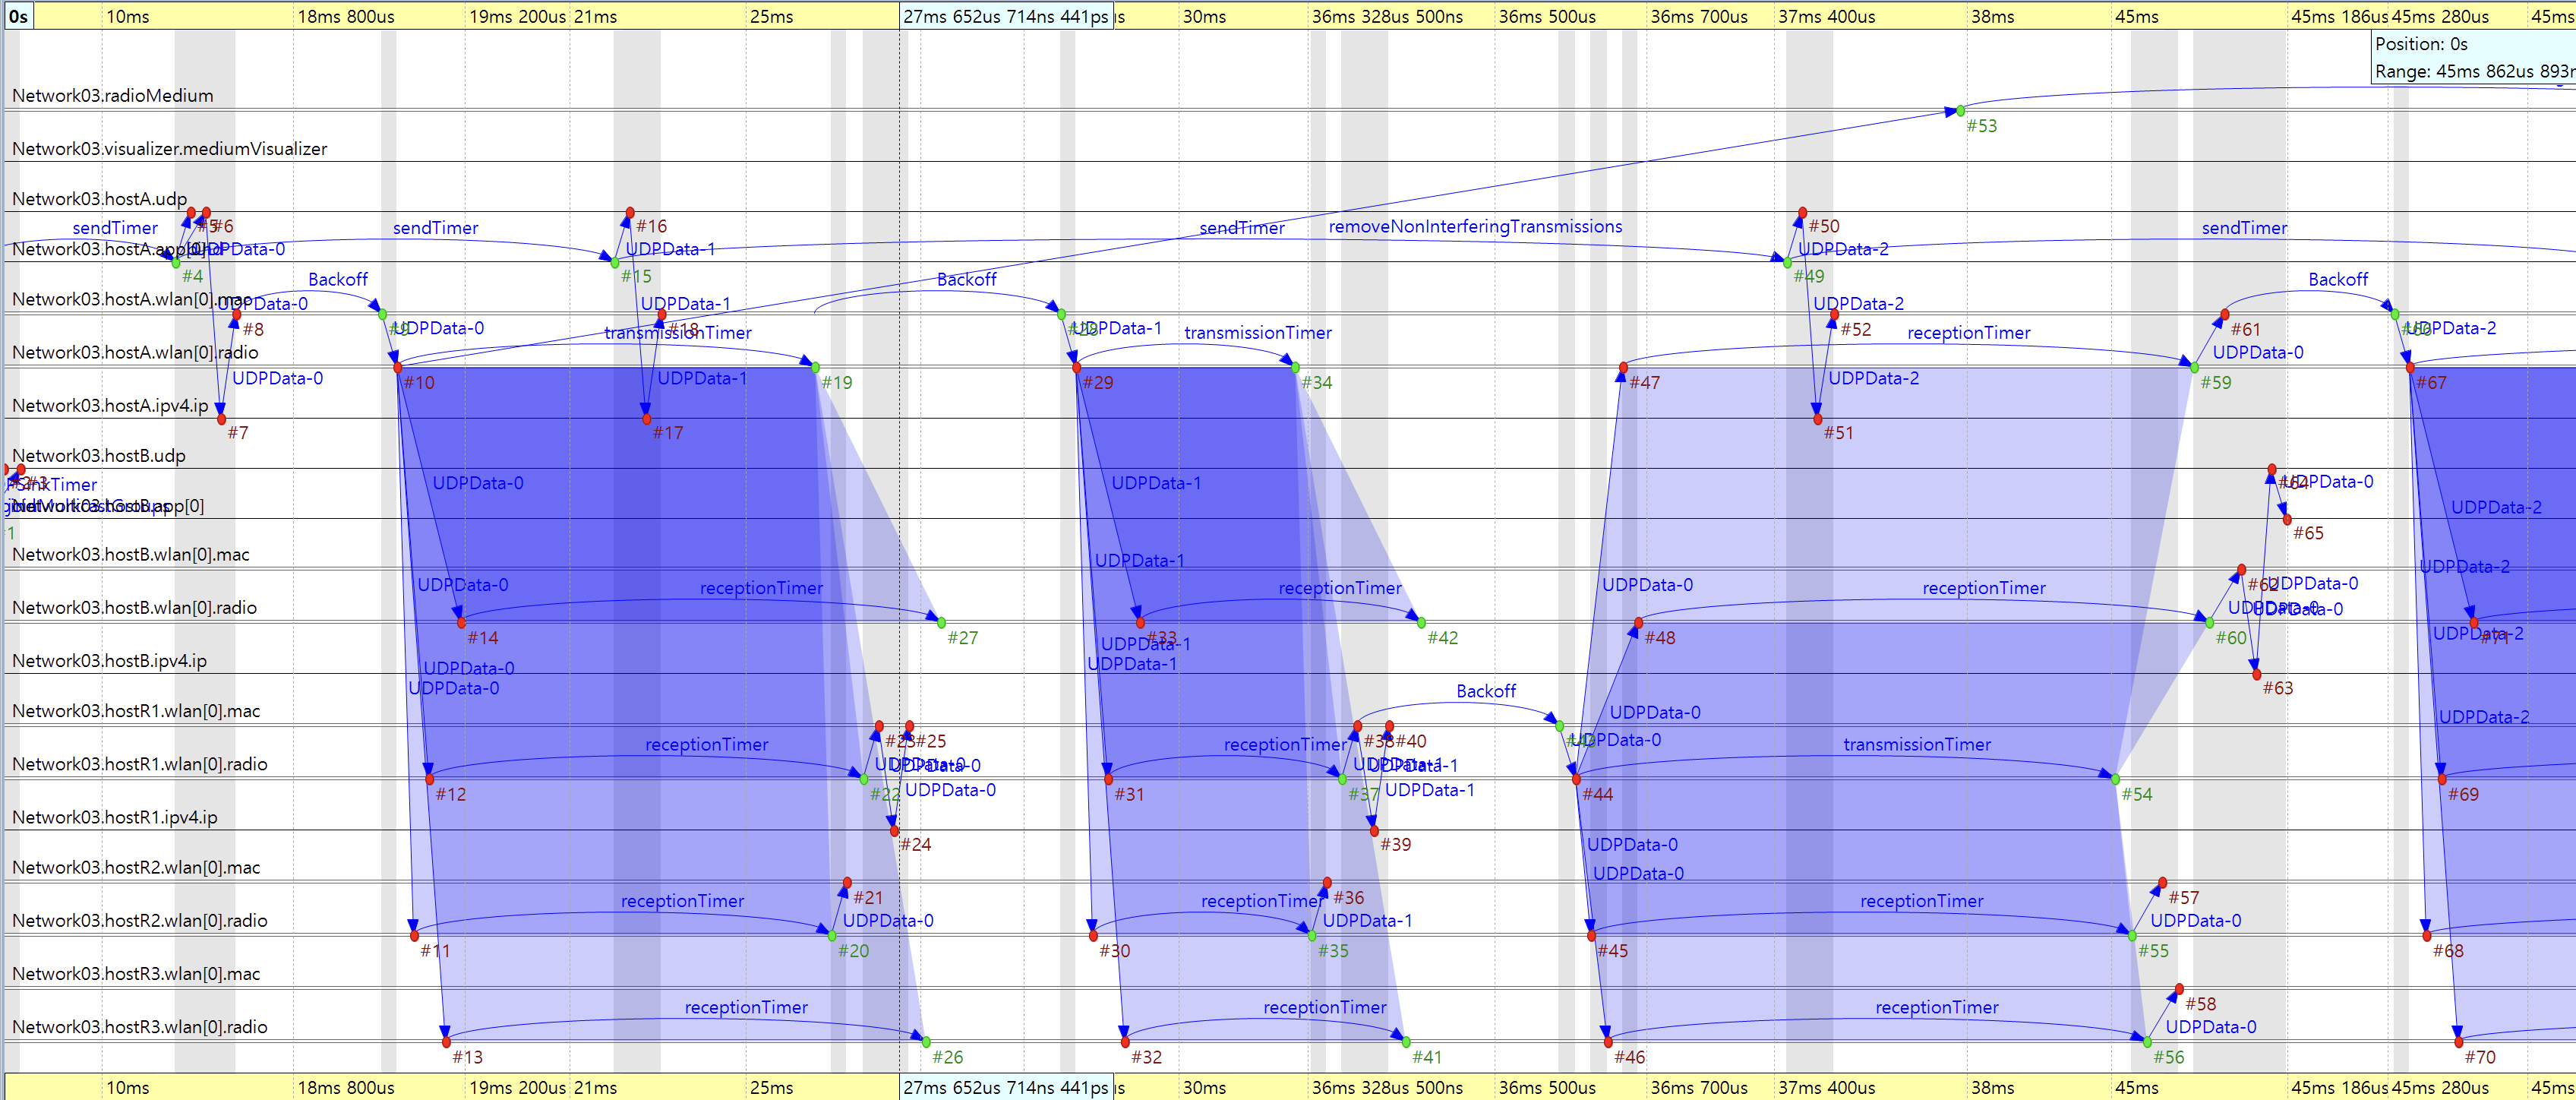
\includegraphics[width=0.9\textwidth]{image/week12/5-1.png}
}\hspace{3mm}
\subfloat[Experiment-4 csma / ca]{
    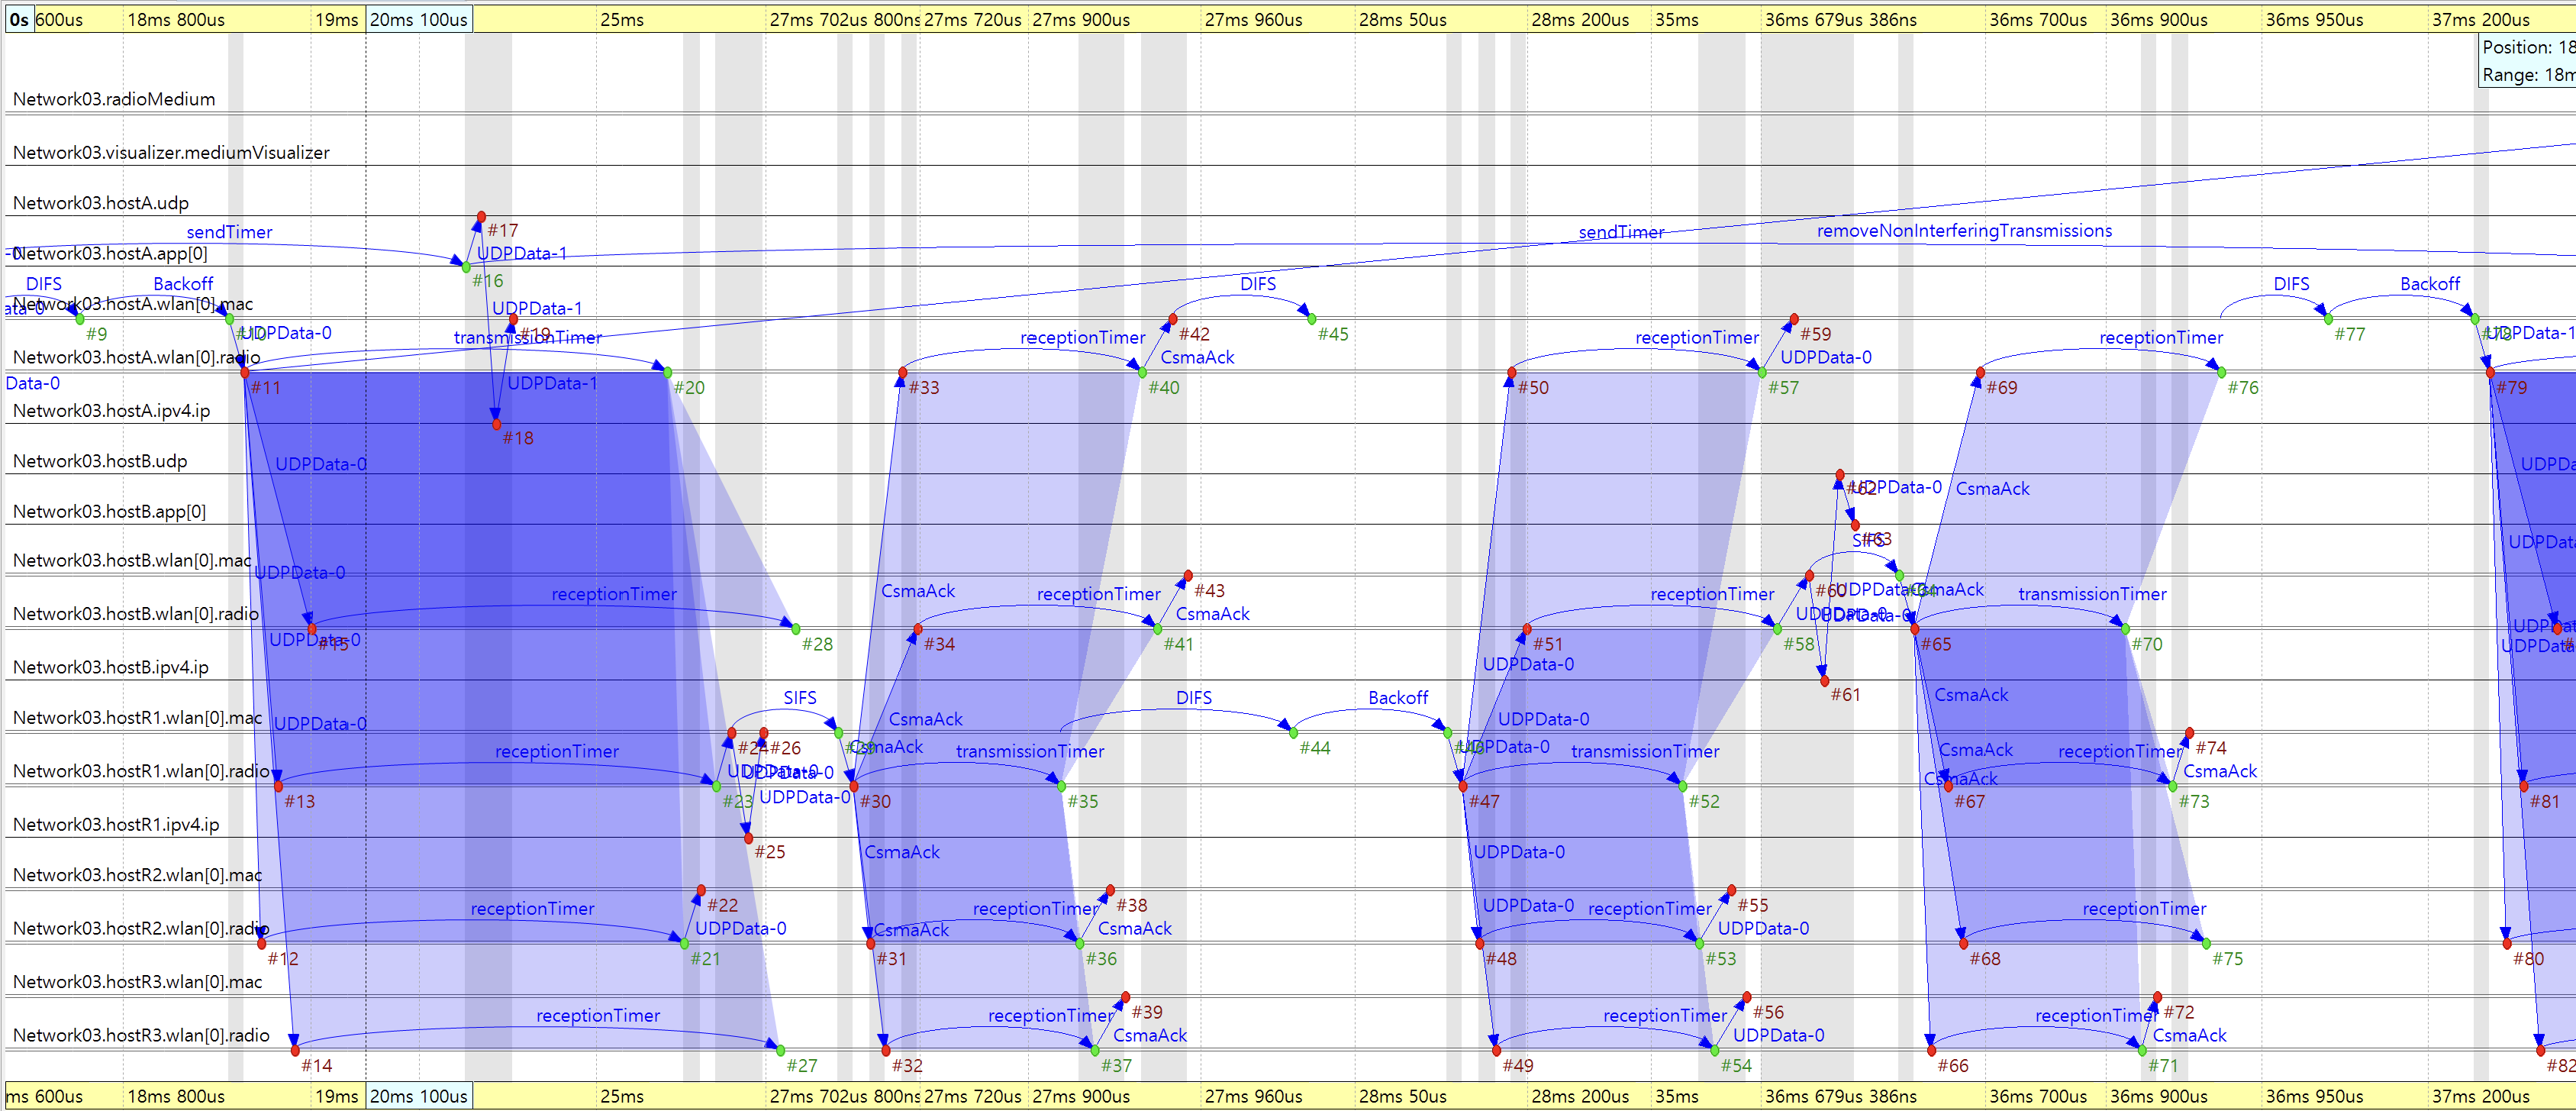
\includegraphics[width=0.9\textwidth]{image/week12/5-2.png}
}
\end{figure}

\clearpage
% \section*{Appendix}
\vspace{-3mm}
\subsection*{omnetpp.ini}
\vspace{-2mm}
\inputminted[framerule = 1pt,framesep = 2mm , frame = lines, fontsize=\scriptsize]{c}{./code/week12/Experiment_05/omnetpp.cpp}
\subsection*{Network02.ned}
\vspace{-2mm}
\inputminted[framerule = 1pt,framesep = 2mm , frame = lines, fontsize=\scriptsize]{c}{./code/week12/Experiment_05/Network02.cpp}
\subsection*{Network03.ned}
\vspace{-2mm}
\inputminted[framerule = 1pt,framesep = 2mm , frame = lines, fontsize=\scriptsize]{c}{./code/week12/Experiment_05/Network03.cpp}
%%%%%%%%%%%%%%%%%%%%%%%%%%%%%%%%%%%%%%%%%%%%%%%%%%%%%%%%%%%%%%%%%%%%%%%%%%
\import{./TEX/week13}{01}
%-------------------------------------------------------------------------
\end{document}